\documentclass[oneside]{ZJUthesis}

% 该文档中首字符为“%”的均为注释行,不会在论文中出现
% 论文默认为双面模式,需单面模式请将第一行换为如下所示:
% \documentclass[oneside]{ZJUthesis}
% \documentclass[twoside]{ZJUthesis}

% 取消目录中链接的颜色,方便打印
% 如需颜色,请将“false”改为“true”
\hypersetup{colorlinks=false}

% 这里几行代码使得目录中的“第几章” 和后面的章节名称不致发生重叠
\makeatletter
\renewcommand{\numberline}[1]{%
\settowidth\@tempdimb{#1\hspace{0.5em}}%
\ifdim\@tempdima<\@tempdimb%
  \@tempdima=\@tempdimb%
\fi%
\hb@xt@\@tempdima{\@cftbsnum #1\@cftasnum\hfil}\@cftasnumb}
\makeatother

%\usepackage[sectionbib]{chapterbib}

\makeatletter
\def\@chapter[#1]#2{\ifnum \c@secnumdepth >\m@ne
  \if@mainmatter
    \refstepcounter{chapter}%
    \typeout{\@chapapp\space\thechapter.}%
    \addcontentsline{toc}{chapter}%
    {\protect\numberline{第 \chaptername 章}\hspace{1em}#1}
%    {\protect\numberline{\chaptername}\hspace{4em}#1}
  \else
    \addcontentsline{toc}{chapter}{#1}%
  \fi
  \else
  \addcontentsline{toc}{chapter}{#1}%
  \fi
  \chaptermark{#1}%
  \if@twocolumn
  \@topnewpage[\@makechapterhead{#2}]%
  \else
  \@makechapterhead{#2}%
\@afterheading
\fi}
\makeatother

\begin{document}
%%%%%%%%%%%%%%%%%%%%%%%%%%%%%
%% 正文字体设定
%%%%%%%%%%%%%%%%%%%%%%%%%%%%%
\songti

%%%%%%%%%%%%%%%%%%%%%%%%%%%%%
%% 论文封面部分
%%%%%%%%%%%%%%%%%%%%%%%%%%%%%
% 中文封面内容

% 中图分类号
\classification{TM391}

% 单位代码
\serialnumber{10335}

% 密级,如需密级则将其前“%”去掉
%\SecretLevel{绝密}
\SecretLevel{公开}

% 学号
\PersonalID{21432041}

\title{基于KECA的非线性故障检测}
% 如果标题一行写不下,就写成两行,在下面的命令里写第二行,不需要两行则注释掉
%\titletl{论文题目第二行}
%\titletl{test}

%英文题目
\Etitle{Nonlinear Fault Detection Based on KECA}
% 如果一行写不下,同中文题目设定,一行写不下则写两行,不需要就注释掉
%\Etitletl{English Title The 2nd Line}
%\Etitletll{}

% 作者
\author{秦家祥}
\Eauthor{Jiaxiang Qin}

\degree{硕士}
\Edegree{Master of Engineering}

% 导师
\supervisor{杨春节~~~教授}
\Esupervisor{Prof. Chunjie Yang  Supervisor}

% 合作导师,如果有的话,去掉注释
% \cpsupervisor{}
% \Ecpsupervisor{}

% 专业名称
\major{控制科学与工程学}
\Emajor{Control Science and Engineering}

% 研究方向
\researchdm{研究方向}
\Eresearchdm{research domain}

% 所属学院
\institute{控制科学与工程学院}
\Einstitute{College of Control Science and Engineering}

%论文提交日期
\submitdate{二〇一六年十二月五二十六日}
\Esubmitdate{2016-12-26}

% 答辨日期
\defenddate{2017-03-10}

% 生成封面
\makeCoverPage

% 生成英文封面
\makeECoverPage

%%%%%%%%%%%%%%%%%%%%%%%%%%%%%%
%% 中文题名页内容
%%%%%%%%%%%%%%%%%%%%%%%%%%%%%%
% 论文评阅人信息 注意两字名与三字名,两字职称与三字职称的写法,便于对齐
% 多余的名额直接注释掉即可,比如三个评阅人,把评阅人D,E注释掉即可
\reviewersA{匿名评审}
\reviewersB{匿名评审}
\reviewersC{匿名评审}
\reviewersD{}
\reviewersE{}

% 答辩委员会信息,如果某一个单位比较长,
% 请在其它较短后面补上{hspace{Xem}},X是比最长的单位名少几个字
% 如果实际人数少于6人,多余的注释掉即可
\chairman{}
\commissionerA{}
\commissionerB{}
\commissionerC{}
\commissionerD{}
\commissionerE{}

% 生成中文题名页
\maketitle


%%%%%%%%%%%%%%%%%%%%%%%%%%%%%%
%% 英文题名内容
%%%%%%%%%%%%%%%%%%%%%%%%%%%%%%
\englishtitle{Nonlinear Fault Detection Based on KECA}
% 如果题名一行写不下,就写到第二行,不需要则将其注释掉
%\englishtitletl{English Title The 2nd Line}
%\englishtitletll{}

% 评阅人信息,名字,职称,单位尽量用简写,否则会写不下
\EreviewersA{anonymous reviewer}
\EreviewersB{anonymous reviewer}
\EreviewersC{anonymous reviewer}
\EreviewersD{}
\EreviewersE{}

% 答辩委员会信息,同样尽量用简写,否则会写不下
\Echairman{}
\EcommissionerA{}
\EcommissionerB{}
\EcommissionerC{}
\EcommissionerD{}
\EcommissionerE{}

% 生成英文题名页
\makeenglishtitle


%%%%%%%%%%%%%%%%%%%%%%%%%%%%%%
%% 原创声明与版权协议页
%%%%%%%%%%%%%%%%%%%%%%%%%%%%%%

\SignautreDateA{2017}{3}{10}
\SignautreDateB{2017}{3}{10}
\SignautreDateC{2017}{3}{10}
% 生成原创声明与版权协议页
\makeOSandCPRTpage


%%%%%%%%%%%%%%%%%%%%%%%%%%%%%%
%% 论文部分开始
%%%%%%%%%%%%%%%%%%%%%%%%%%%%%%
\ZJUfrontmatter

%%%%%%%%%%%%%%%%%%%%%%%%%%%%%%
%% 勘误页,一般没有
%%%%%%%%%%%%%%%%%%%%%%%%%%%%%%
\begin{corrigenda}
这是一个勘误\index{勘误}章节,一般情况下是没有的。
\end{corrigenda}



%%%%%%%%%%%%%%%%%%%%%%%%%%%%%%
%% 序言页,一般没有
%%%%%%%%%%%%%%%%%%%%%%%%%%%%%%
\begin{preface}
上一版发布于2011年10月26日,发布之后的近两年来,陆陆续续收到一些邮件问关于使用中的一些问题,
我也算基本上做到一一解答。
同进也在着手准备根据提到的问题对这一版模版进行一定的修订,增补一些使用中普遍关心的难点问题。
因为事务冗杂缠身,加上关于参考文献格式调整部分的内容一直没有时间看明白,这个事情就一直拖下来了。
直到前一段断断续续看完了参考文献格式整理部分的帮助资料,搞清楚了它的实现思路原理,
才算又着手修订这一版教程。

在这过去的一年多里,接触到了\XeTeX{},对其强大的直接调用系统字体的能力表示赞叹,
于是将这个模版切换到了\XeTeX{}的环境下,将文件代码换成了对多语言兼容更好的UTF-8代码,
但同时保留对GBK码的兼容,具体不同之处会在后面的章节中提到。
因此新的一版分为UTF-8和GBK两个版本进行发布,两个版本使用上只有很细微的区别,
一般使用过程中可以忽略这个差别。

以下是原来的序言,此处照旧附上。


很早就听说过\LaTeX\index{\LaTeX}了,但却一直没有真正学习过,直到今年,需要处理一些大文档,想起了\LaTeX{}。
重新翻出\LaTeX{}的文档,从CCT开始,至于为什么是CCT,
因为Ctex\index{CTeX}提供的那个CTeX FAQ里对中文的第一个例子,就是以CCT
为例写的。
CCT是中科院的张林波研究员写的,帮助文档都是中文,看起来比较容易,但毕竟是好几年前的版本了,
更新也并不是那么及时,而且CCT\index{CCT}早期版本的字体是点阵字体,边缘很粗糙,
虽然不影响打印,但在这个年代还在用着这样的字体,着实不是那么舒服。
我又开始了第二个例子,CJK的尝试,在尝试CJK\index{CJK}的过程中,
无意中看到了CTeX的ctexart,ctexbook和ctexrep这几个基本模版,这才找到CTeX的门,
筒子们不要笑我绕了这么一大圈才摸进了CTeX的门,虽然从开始就使用的是CTeX的发行版。

这里也要说一下,CTeX提供的部分帮助文档内容也比较老了,一些操作现在新的软件虽然仍然兼容,
但已经不是新版软件推荐的做法了,比如,CTeX FAQ里面对于pdf文件的生成,
依然是先由latex.exe生成dvi文件,再由dvi文件生成ps文件,最后再生成pdf文件。
实际上,现在流行的新版\TeX{}类软件都已经将pdfTeX\index{pdfTeX}作为默认引擎,支持直接生成pdf文件,
而且dvi、ps文件的打开速度比pdf反而要慢许多。我使用的是64位系统,CTeX提供的安装包只支持32位系统,
我单独安装的MikTeX\index{MikTeX} x64\index{x64}版使用CTeX模版生成的dvi文件使用dvips\index{dvips}处理时会找不到字体,
因为这个问题,我找了很久,最后的结论是:dvips可以放弃了,直接使用dvipdfm\index{dvipdfm}更合适。

后来几天在\LaTeX{}的实践中看不少相关细节,开始对其模版产生了兴趣,
在88上\TeX{}版把置顶的ZJUthesis下了下来,就是写这个模版的基础,数学系模版。
下下来后发现这个模板给的例子pdf与当前学校使用的2008年论文模版差别老大了,从封面到目录,
章节格式,都是完全不一样,因此,决定着手做一个与学样提供的Word模版比较接近的模版。

在以2006年数学系模版为基础进行新模版编写的过程中,学了不少方法,
也发现老模版不少过时或者不合适的地方。
第一个学到的就是,从模版一开头就发现这个模版是以ctexbook这个模版为基础制作的,
做到模版完成的时候,
发现88的\TeX{}版置顶模版已经更新,我以为我白做了,
下下来一看,原来这个新的模版不是以ctexbook为基础制作的,而是更基础的\LaTeXe\index{\LaTeX}
对比自己基本完工的模版,才发现ctexbook为我省了很多工作量。只是一些修修改改就做到了很接近学校
word模版的效果。
ctexbook的新版已经直接将hyperref包打了进去,2006年数学系模版对hyperref\index{hyperref}的引用判断部分已经明显示过时,在用新版MikTeX运行的时候直接报错了。
在编写封面的时候,发现2006年的模版用了一个五列的表格,可这部分的内容只需要两列就够了,
直到我某天下载了中科院的模版后才明白,2006年版模版是从中科院模版改编而来,
中科院模版在封面上名字等内容的排列方式需要采用五列表格。这一部分,我也将其重新编写。

随着时代的推进,\LaTeX{}的各种功能包日渐丰富,很多过去只能从\LaTeXe{}代码写的功能,
如今可以通过相应的功能包直接实现,在这个模版中,我使用了几个新的功能包,
其中最新的当属刚刚发布的hyperref更新包,增加了hidelinks命令,可以直接将链接的边框去掉,
不用采用将边框颜色设为白色的方式了。

就像\LaTeX{}的版本总是在接近$\pi$的值一样,这份模版并不是完美的,比如对数学系的定理体系支持不足,
留在以后版本再发布或者请有兴趣的爱好者共同修改。编写这一版本的基本目的是没有任何\LaTeX{}基础的同学可以比较轻松地利用它给自己的毕业论文排一个满意的版面,整个模版没有留太多选项,
可供修改的选项只有两个:单面双面的选择和链接的颜色的有无。在模版中,我对绝大多数的语句,
都做了中文注释,解释其作用,方便有兴趣的同学研究,我也是一个初学者,作出的这份模版,
我想,应该是比较适合初学者胃口的。

\end{preface}


%%%%%%%%%%%%%%%%%%%%%%%%%%%%%%
%% 摘要
%%%%%%%%%%%%%%%%%%%%%%%%%%%%%%
\begin{abstract}
这份文档主要介绍了该\LaTeX{}论文模版的使用方法,注意事项,一些使用技巧。

另外,这份文档的源代码修改自shuwei1204@163.com的google code项目,该项目的下载地址为:http://code.google.com/p/zjuthesistex/downloads/list。

\keywords{\LaTeX,论文模版,ZJU}
\end{abstract}

{\pagestyle{empty}\mbox{}\newpage\pagestyle{empty}}  % 无页眉页脚的空白页
%%%%%%%%%%%%%%%%%%%%%%%%%%%%%%
%% 英文摘要
%%%%%%%%%%%%%%%%%%%%%%%%%%%%%%
\begin{englishabstract}
The quick brown fox jump over the lazy dog.

\TeX\index{\TeX}

\englishkeywords{\TeX}

\end{englishabstract}

{\pagestyle{empty}\mbox{}\newpage\pagestyle{empty}}  % 无页眉页脚的空白页

%%%%%%%%%%%%%%%%%%%%%%%%%%%%%%
%% 论文部分开始2
%%%%%%%%%%%%%%%%%%%%%%%%%%%%%%
\ZJUfrontmatterTwo

%%%%%%%%%%%%%%%%%%%%%%%%%%%%%%
%% 目录页
%%%%%%%%%%%%%%%%%%%%%%%%%%%%%%
\ZJUcontents

%%%%%%%%%%%%%%%%%%%%%%%%%%%%%%
%% 插图列表
%%%%%%%%%%%%%%%%%%%%%%%%%%%%%%
\ZJUListofFigures

%%%%%%%%%%%%%%%%%%%%%%%%%%%%%%
%% 表格列表
%%%%%%%%%%%%%%%%%%%%%%%%%%%%%%
\ZJUListofTables

%%%%%%%%%%%%%%%%%%%%%%%%%%%%%%
%% 缩写、符号清单、术语表
%%%%%%%%%%%%%%%%%%%%%%%%%%%%%%
\begin{ListofSymbol}
缩写、符号清单、术语表
\end{ListofSymbol}


%%%%%%%%%%%%%%%%%%%%%%%%%%%%%%
%% 正文内容部分开始
%%%%%%%%%%%%%%%%%%%%%%%%%%%%%%
\ZJUmainmatter

\chapter{简介}

\section{为什么}

“为什么用\LaTeX{}{}?”

当把\LaTeX{}{}介绍给一个人的时候,这是面对的第一个问题。
当回答“它很好用时”,又会得到第二个问题:
“Word不好用吗?”答案当然是肯定的,
Microsoft Word\index{Word}是这个世界上目前最流行的,最易用的文字处理软件之一。

但是,
我这里要做一个转折了,如果是做过比较大的文档的,几十页以上,有分章,
分节,或者还要有页眉页脚页码目录以及封面这些东西,好吧,大部分人做过唯一的这种文档,那就是毕业论文了。
给毕业论文排版,几乎是大部分人的一场梦魇。如果性格里再带一点点追求完美的
念头,追求一点点排版的质量,那给自己的毕业论文排版,那一定会留下一生深刻的印象!

页码格式不对,页码编号不对,不同章节标题字体不一致,小标号缩进老对不齐,
数字有时候是Times Roman字体,
有的时候又成了宋体,有的段落前有一块空白,有的段落间距又太小。增加了一张图,
它后面图的标号又得重新来编一次,还有图的引用处也不要忘记……增加了一段文字,发现排好
的图又跑到下面一页去了。。。。。这一页留下了好大一片空白。下一页的表格又被它推
成了分布在两页。参考文献引用增加或者删除了一个,那就得找出全文要改动的所有引用处!!
什么,你是高级用户,会使用交叉引用,好吧,那有时候打出来的文档突然出现“错误!找不到引用--”
这样的字样,你是什么心情?
生成目录字体不一样,有的标题起的名太长,把页码挤到下一行去了,一个个改好了,一全更新又完了。
如果你的文档里还有一些公式,那又是一场战争了,有的公式字显得比正文大,有的又显得比正文小,
或者总是跟写的编号对不齐,不是偏上就是偏下。公式编辑器\index{公式编辑器}版本众多,换台电脑就只能看不能改了,
公式编辑器还经常提示已过期。blablabla……

千辛万苦,终于搞定了,看起来还算漂亮,到打印店去了,omg,word版本不对,版白排了,又乱了。
用PDF吧,不同软件生成的PDF总是跟原来的样子有点差距。做完论文,感觉是扒了一层皮。

\LaTeX{}解决了这个问题,它实际可以看成是一种写给机器的语言,把格式定义好,再填上内容,
它就会按设定好的格式把一份文档生成出来,一般是生成pdf文档,整个文档的格式首先是统一的,
不会出现不同章节的显示不一样的问题,并且,文档的格式可以是封装好的,使用的时候不需要
理会具体格式,直接可以使用,封闭格式这个功能留给会的人去做,写论文不需要关心太多的格式问题。

如果是往国外投文章,那么\LaTeX{}的应用更广泛,不少国外出版社直接提供其格式文件,
只要将文档头上的$\backslash$documentclass\{article\} 大括号里的“article”换成其相应的格式文件即可,
避开了格式调整问题。

话说回来,Word还是有优势的,所见即所得,上手容易,会鼠标键盘就会用。\LaTeX{}还是需要一些入门时间的,
如果单纯会使用这个模版,我想大约需要3个小时左右,如果会处理一些常见的程序错误以及做小的格式修改,
时间就会比较长了,大约要几天,有人引导的话会快一些。
Word在做小文档,比如就几页的文档上的优势\LaTeX{}{}是无法与之比拟的,做起来是很快,比如通知啦,传单啦。
但Word存在的意义应该不是就为了那几张小广告的,几百M的体积,几百RMB的价格,当然盗版很多。在这种应用
上还不如去用一下免费的WPS,或者OpenOffice。Word支持很多特性,支持宏,支持Visual Basic……,但是,它们
又太难了,不是随便一个人就会去有兴趣学它们的,学了很少有机会用到,屠龙之技。

\LaTeX{}{}还有两个优势是Word所没有的:
\begin{enumerate}
\item{文件体积小}

使用\LaTeX{}{},所要编辑的文件以“tex”为扩展名,如果用到参考文献,可能还需要扩展名为“bib”的参考文献数据库
文件,此外,还可能有的就是文档中要插入的图片文件了。
“tex”和“bib”文件都是纯文本文件,如果愿意,可以用记事本来编辑,按照一定的格式书写,格式也是很简单的,
看到了就会使用。
而Word文件是Microsoft自己定义的二进制文件,只有用Word软件或者其它兼容的软件打开,因为是Microsoft自己的二进制格式,
因此,体积会比较大,当然文件集成度很好,只有一个文件。
相比较之下\LaTeX{}{}可能有很多文件,但这个缺陷完全可以通过压缩软件打包来完成。
如果打开一个比较大的文档,机器破的话会比较慢,而且容易出一些错误导致Word意外关闭,想来各位都遇到过这种情况的吧。
文件如果发生了意外关闭,那就有可能被损坏,损坏后就有可能。。。。。打不开了,如果没有做一些备份,
那就成了“杯具”甚至“餐具”了。相较而言,\LaTeX{}{}的文件小,而且是纯文本文件,即使被损坏,
修复起来也比Word要容易得多。

\item{使写作更加专注于内容}

说实话,这一条在学会使用\LaTeX{}{}之前,我觉得是扯淡,那时的我觉得,使用Word边写边想也一样很快的。但在我学习使用\LaTeX{}{}
的过程中,我逐渐感受到,当只面对文本,不去想它下一段怎么排,什么样的格式时,思维更加连续,写起来也更快,
而且明显感觉到自己进入了一种写作的状态,这种感觉只在以前纸上写作感觉得到,专注于自己想的内容。
这一点,只有在学会使用之后,才能去体会得到。

\end{enumerate}

\section{模版简介}

该模版以CTeX社区发布的ctexbook模版为基础,在数学系2006年模版上修改而来,删除了不兼容的旧代码,
增加了一些新版本扩展包支持的高级命令,部分功能实现方式与旧版有所不同。

该模版与研究生院网站发布的2008年模版排版效果基本相似,可直接使用。

该模版非学校官方模版,该模版可能引起的问题,{\bfseries{}模版作者不承担任何责任},特此声明。

\subsection{\LaTeX{}{}简介}

\LaTeX{}不是单指一个软件,而是指一类软件,这一类软件都是以一个基本软件\TeX\index{\TeX}为基础,
制作成宏包并经\TeX{}的原作者授权后发布。
打个比方,\TeX{}就是一些方形,三角形,圆形,半圆形的积木块,
\LaTeX{}就是另一些人用这些积木块搭成小房子,小桌子,
我们再把这些做好的小房子,小桌子摆摆成为我们的积木城市群,
就是这样。

为了国际化,\TeX{}不读“太可斯”,而按原作者Knuth, Donald Ervin的说法,
应读为“太chi”\cite{LaTeXshzh}。

Kunth是一个计算机与数学家,\TeX{}是其在1977年看到自己的成果出版时印刷质量甚不满意,
于是历时5年编写了\TeX{}排版系统,这成为西文排版业的一次重大革命。
\TeX{}系统于1982年正式定型,不再做大的改进,只修正发现的错误。
1989年,\TeX{}系统做了迄今为止最大的一次改进:支持多语言\cite{LaTeXshzh}。

\TeX{}的设计思想很简单:把一张纸看成一个坐标平面,将该坐标平面上哪一点要出现的内容标记出来,
就像这样:坐标(50,50),放置一个五号宋体的字,倾体,不加粗;从坐标(80,50)到坐标(80,200),
画一条粗为2的线,黑色……一个排好的版面就是这样被一个点一个点描述地画出来,Knuth设计的
\TeX{}指令,就是这些描述指令,然后由计算机解读,并做出最终的图,就是我们看到的排版效果。
\TeX 的精度很高,它的最小尺寸是一个叫做sp的小单位。可见光的波长近似等于100 sp,
几个sp 的误差眼睛是看不出来的\cite{texbook}。

从上面不难想到,如果只用\TeX 指令进行排版的话,会比较复杂,普通人难以胜任。
作为计算机专家的Knuth很清楚这一点,他给\TeX 设计了扩展接口。
利用这些接口,可以把\TeX 的一系列命令封装起来,做成各种各样的“宏”,这些宏,就被称为\LaTeX{}。
就像上面的比喻一样,用积木做小房子,小桌子的厂家有很多,于是就有了各种各样的\LaTeX{}版本:
MiKTeX,XeTeX,TeXLive,teTeX,fpTeX等。
使用\LaTeX{}模块,使得排版成为一件容易的事,尤其是使用已制作好的模版写文章,
不需要任务基础,知道几条语句就可以排出整齐统一的版面。
使用哪个版本的\LaTeX{}没有关系,都可以使用这个模版生成论文。这个模版制作使用的LaTeX版本是MiKTeX 2.9版。

\subsection{模版内容}

按照研究生院提供的2008版模版,毕业论文一共由封面、题名页、版权声明、勘误表、
致谢、序言、摘要、图表目录、术语表、目次、正文、参考文献、符录、索引、简历、文章列表,
一共十六部分组成\footnote{其实,还有脚注没有算上,脚注是隐含的,在这里\LaTeX{}将主动替你完成脚注的插入,而无需多作分心。就像这个脚注一样。}。

本模版将图表目录分成了图片目录与表格目录两个部分,因为这样一来清楚,二来\LaTeX{}原生支持图片与表格
分开作目录,作到一起反而费事。其它部分与研究生院模版相同。

在该模版中,任何一个部分都是可自由选择有无,如勘误表,大部分论文是没有这个部分的,
不需要某部分,只要将其生成语句注释掉即可,具体将在后面章节中讲解。
使用该模版,封面、题名页、版权声明、图片目录,表格目录、目次、参考文献、索引这八个部分不需要论文
作者直接参与,只需按要求在文中作出标记,\LaTeX{}就会替你自动生成这些部分,
而且完全不必考虑条目的编号顺序等问题。




\chapter{软件环境及设置}

该模版是基于CTeX社区发行的ctexbook模版,因此要使用该模版需要有CTeX环境。

与第一版稍有不同的时,由于该版提供了采用UTF-8编码的\XeTeX{}引擎的新版本和使用原有采用GBK编码的\LaTeX{}引擎的老版本,
因此,如果使用新版本,还需要参考本模版文件包中提供的ctex-xecjk-winfonts.def文件将自己系统中的
ctex-xecjk-winfonts.def文件进行修改,
该文件位于ctex目录下的$\backslash$tex$\backslash$latex$\backslash$ctex$\backslash$fontset目录下。
需要至少指定以下六种字体对应的字体文件:
\begin{verbatim}
\setCJKfamilyfont{zhsong}{SimSun}
\setCJKfamilyfont{zhhei}{SimHei}
\setCJKfamilyfont{zhkai}{KaiTi}
\setCJKfamilyfont{zhfs}{FangSong}
\setCJKfamilyfont{zhli}{LiSu}
\setCJKfamilyfont{zhyou}{YouYuan}

\newcommand*{\songti}{\CJKfamily{zhsong}} % 宋体
\newcommand*{\heiti}{\CJKfamily{zhhei}}   % 黑体
\newcommand*{\kaishu}{\CJKfamily{zhkai}}  % 楷书
\newcommand*{\fangsong}{\CJKfamily{zhfs}} % 仿宋
\newcommand*{\lishu}{\CJKfamily{zhli}}    % 隶书
\newcommand*{\youyuan}{\CJKfamily{zhyou}} % 幼圆
\end{verbatim}

其它字体可以自由指定,SimSun,SimHei这些指定字体的关键字可以直接用字体文件*.ttf 来代替,
也可以使用命令“fc-list”来具体查看系统中已安装的字体的名字,从而对应地填到上述命令中去。


\section{Windows系统}

Windows系统下可以直接安装CTeX发行的软件包,该发行包只有32位版本,64位系统安装方法与32位略有不同。下面分别介绍。

\subsection{32位系统}

包括windows XP,Windows Server 2003,Vista, Windows Server 2008 和 Windows 7。

32位系统下安装比较简单,直接从www.ctex.org下载最新的安装包,当前最新版为2.9.2.164,
它包括CTeX环境,winEdt,MiKTeX,Ghostcript,几个部分,除CTeX环境外,
另外几个组件都可以选择安装,如可以用TeXLive替代MiKTeX,UltraEdit,gvim,Emacs替代winEdit等。
如果你不了解这几个软件,那么就默认安装选项即可。

安装完后,需要对\LaTeX 软件进行升级,如MiKTeX软件进行升级,升级的网络站点就选中科大的CTAN镜像站,
网址http://mirrors.ustc.edu.cn/CTAN,在教育网内速度还是比较快的,如图\ref{set1},\ref{set2},\ref{set3}所示。

\begin{figure}[th]
\centering
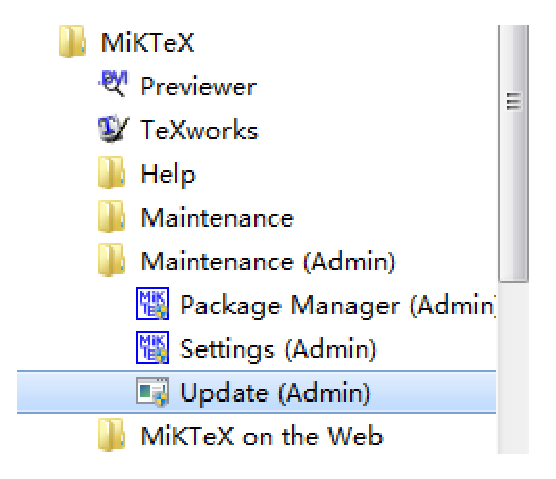
\includegraphics[scale=0.5]{./Pictures/set1.eps}\\
\caption{MiKTeX升级设置}
\label{set1}
\end{figure}

\begin{figure}[th]
\centering
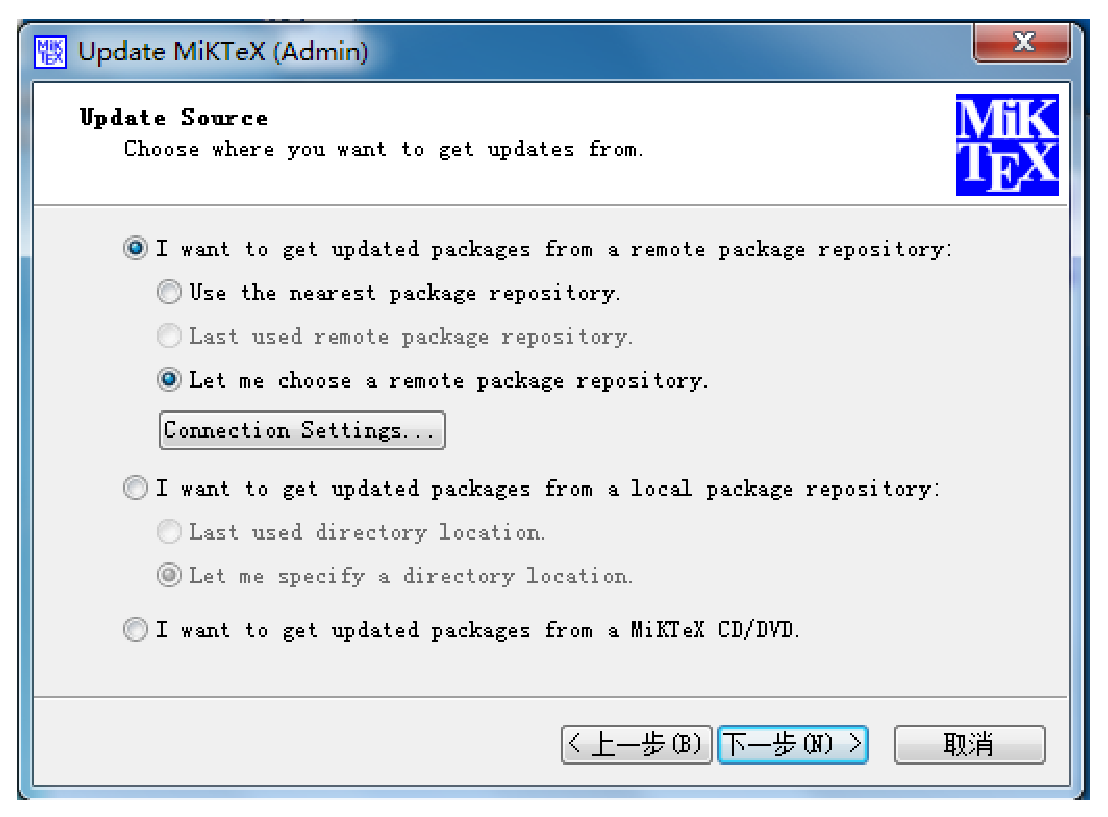
\includegraphics[scale=0.5]{./Pictures/set2.eps}\\
\caption{选择升级方式,如图中选择一个升级站点}
\label{set2}
\end{figure}

\begin{figure}[th]
\centering
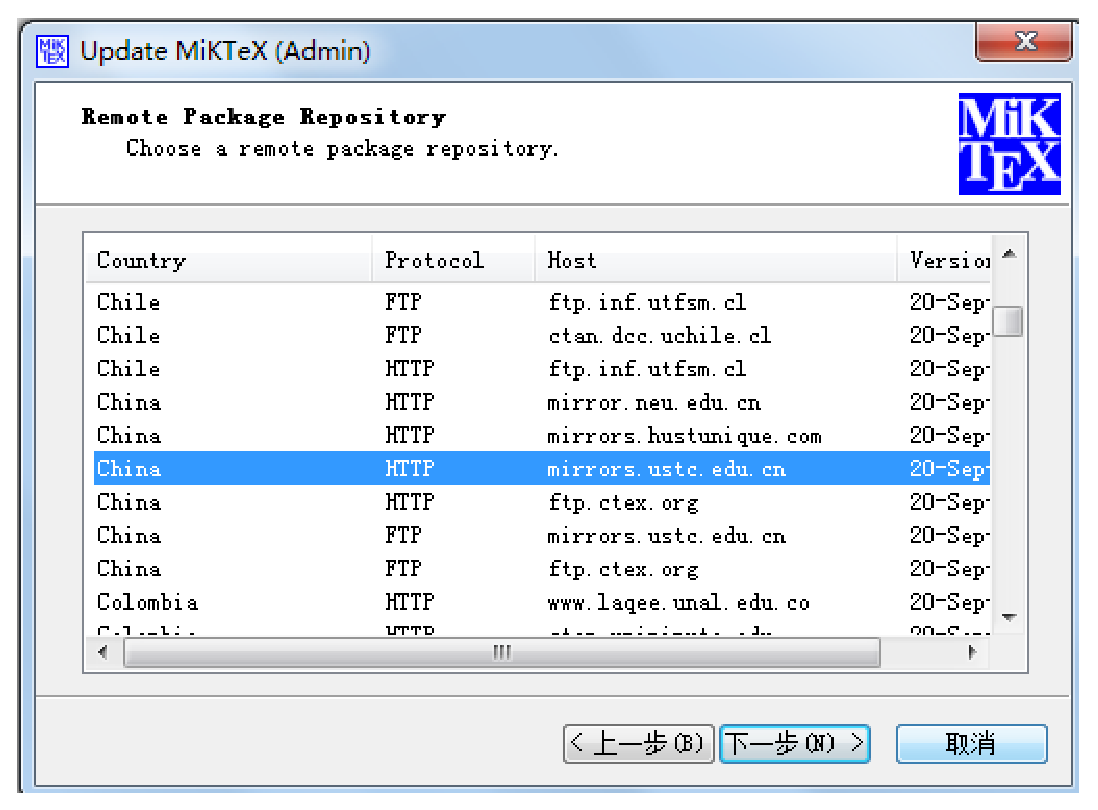
\includegraphics[scale=0.5]{./Pictures/set3.eps}\\
\caption{选择升级站点,以中科大镜像点为例}
\label{set3}
\end{figure}

之所以要把软件升级到最新是因为该模版使用了最新的hyperref包中添加的命令hidelinks。

\subsection{64位系统}

包括windows XP 64bit,Windows Server 2003 64bit,Vista 64bit,
Windows Server 2008 64bit,Windows 7 64bit 和 Windows Server 2008 R2。

安装CTeX安装包时,不要选择MiKTeX,其它软件任意,与32位一样。
安装完CTeX包后,去www.miktex.org网站下载MiKTeX的最新64位版,当前是2.9版,
安装后在设置页面中把CTeX的目录加到MiKTeX的Root目录中去,如图 \ref{setroot} 。
再如图 \ref{rffndb} 所示,刷新MiKTeX的目录数据库,就可以使用CTeX的环境了。

\begin{figure}[thp]
\centering
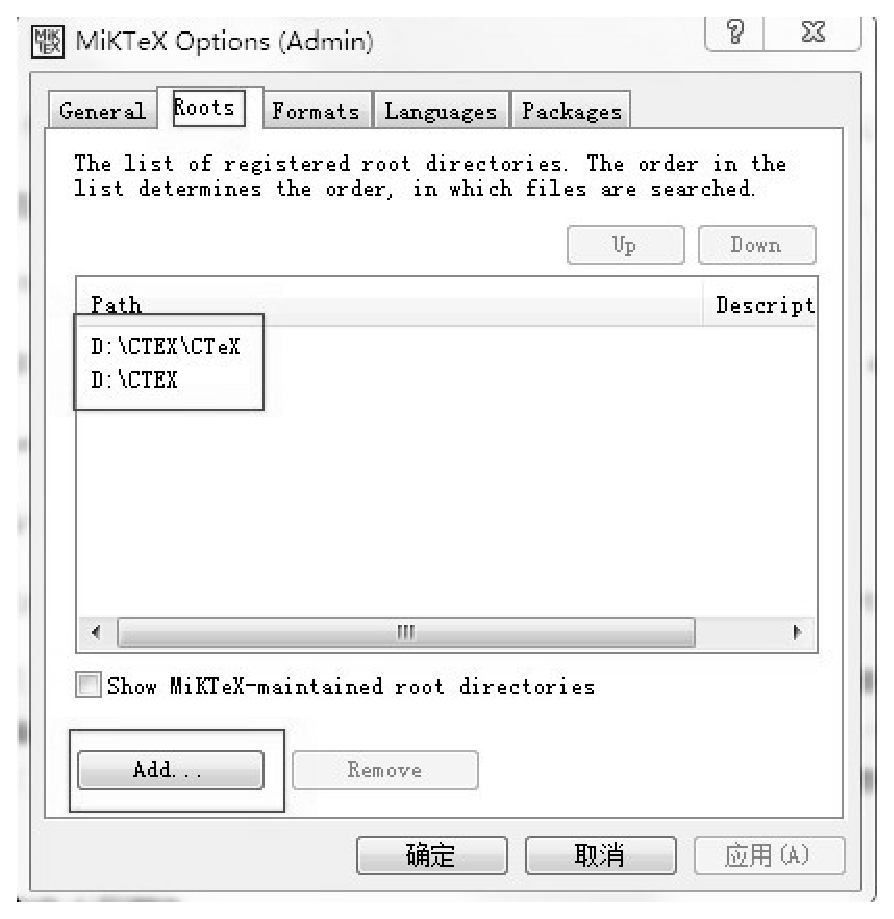
\includegraphics[scale=0.5]{./Pictures/setroot.eps}\\
\caption{设置MiKTeX软件的Root目录}
\label{setroot}
\end{figure}

\begin{figure}[th]
\centering
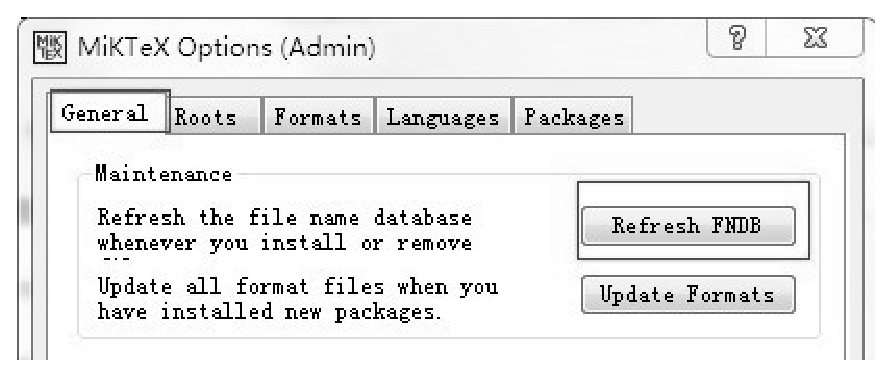
\includegraphics[scale=0.5]{./Pictures/rffndb.eps}\\
\caption{刷新MiKTeX的目录数据库}
\label{rffndb}
\end{figure}

与32位Windows系统相同,安装完后也需要把MiKTeX升级到最新。

\section{linux系统}

请自行选择\LaTeX 安装版本,然后把CTeX环境加入即可。我想用linux的应该都会这个吧。
本次版本使用的操作系统及软件环境是Debian 6和TeXLive2009。

请保证扩展包版本足够新。尤其是hyperref包,保证是2011年8月份后的版本。

\section{Mac系统}

请自行选择\LaTeX 安装版本,加入CTeX环境。同linux下。

\section{本模版所需要的扩展包}

\begin{enumerate}

\item{图形、表格类扩展包} graphicx,array,booktabs-de,caption,natbib,multirow

\item{字体类扩展包} times(\LaTeX{}引擎中用),fontspec(\XeTeX{}引擎中用)

\item{目录选项扩展包} tocbibind,tocloft,makeidx,hyperref

\item{数学公式扩展包} amsmath,amsthm,amsfonts,amssymb,bm

\end{enumerate}

\section{测试运行}

如果已经安装好了CTeX环境与\LaTeX 软件,那么,可以运行这个模版文件包里的makethesis.bat文件,
几秒钟到十几秒后,如果生成了一份叫做“README.pdf”的文档,那么,恭喜,这个模版所需要的软件环境建立成功!
如果没有生成这一份文件,那么有可能你的软件环境没有配置正确,比如把\LaTeX 软件升级到最新,
这份模版所需要的扩展包没有被安装,请打开\LaTeX 软件自动升级功能,
保证\LaTeX 软件能够成功地连接到CTAN站点下载所需的扩展功能包。


\chapter{基于集成学习和贝叶斯推论的改进核熵成分分析}

\noindent \textbf{摘要}\quad 故障检测是故障诊断的一个重要组成部分,通过对故障进行检测,可以有效地判断工业生产过程中是否有故障发生,从而便于展开故障分类、故障隔离及故障重构等。KECA作为一种新的处理非线性的方法逐步地被引入到故障诊断领域,可以利用该方法实现故障检测。本章将集成学习和贝叶斯推论引入到核熵成分分析中,通过集成具有不同参数的学习算法,利用贝叶斯推论将这些算法的检测结果转化为概率的形式实现故障检测。本章提出的新方法在田纳西-伊斯曼过程(TE Process)上进行了应用,并与在相同条件下的单模型KECA 进行检测效果对比,验证了本章提出的新方法对不同类型的故障均具有较好的检测效果,从而说明了新方法的可行性。\\
\textbf{关键词}\quad 故障检测;非线性;集成学习;贝叶斯推论;KECA

\section{引言}

PCA是一种广泛被使用的过程监测方法,该方法通过提取过程当中的主要成分来达到降维的目的,而这些主要成分则是通过数据的方差的大小来反映。然而,在提取主成分的过程中的前提条件是数据服从高斯分布并且假设过程为线性过程。这些前提条件使得PCA针对非线性过程实现过程检测时很难获得满意的监测效果,由此引入了核函数,利用核函数可以将原始的非线性的数据映射到一个高维甚至无限维的空间当中,此时的数据近似为线性。其效果如 \ref{Fig2D3D} 所示。
\begin{figure}[htb]
\centering
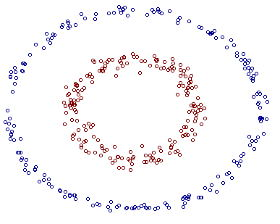
\includegraphics[scale=0.6]{./Pictures/kernel2D.jpg}
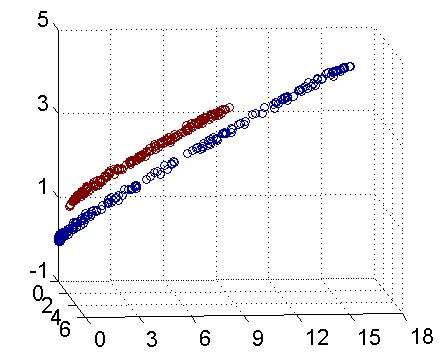
\includegraphics[scale=0.6]{./Pictures/kernel3D.jpg}
\caption{两类数据分别在1)二维空间 ~~~ 2)三维空间}
\label{Fig2D3D}
\end{figure}
从图\ref{Fig2D3D}中可以看出,在二维空间中不可分的两类数据,投影到高维空间利用坐标轴旋转可以实现分类,也就是说利用核函数将数据投影到高维空间后可以找到超平面将原来不可分的数据实现分类,这样就可以实现将非线性问题近似线性化。
这就是KPCA 的出发点,该方法也是最常见的一种处理非线性的方法。
为了更好地将这种方法应用于过程监测当中来,Lee 等人提出了平方预测误差(SPE)的计算方法,由此,$T^2$和SPE 两个统计指标被用到KPCA当中来检测过程。
然而,这两个统计指标的置信限计算方法都是假设输入数据服从高斯分布,但是考虑到过程的非线性这种假设在实际的生产过程当中并不能很好地被满足。
Ge 等人将统计局部方法引入KPCA 中,利用统计局部方法通过假设检验重新构造了两个检测指标,新的构造的检测指标能够较好的满足高斯分布,从而使得故障的检测率较高地提高。
Samuel等则是利用核密度估计(KDE)的方法计算监测指标的控制限,这也在一定程度上改善了监测质量,然而,这也是建立在一定的假设基础上的。
但是KPCA应用于过程检测时,依旧需要满足的假设条件是数据服从高斯分布,
该假设在实际的生产过程中是不可能满足的,
而KECA则是从信息熵的角度出发,不再要求原始数据服从高斯分布,从而与KPCA 相比有更好的检测效果。\\
KECA的原理与KPCA有所不同,在KPCA中考虑到方差对应于数据的特征幅度变化方向,
降维则是通过尽可能多的保留数据特征变化来实现,也就是要通过保留核矩阵最大的方差来实现;
而KECA则是通过引入信息熵的概念,通过保留最大的信息熵来实现姜维的目的。
熵则是通过核矩阵利用Parzen窗实现其密度估计,此时,通过将数据投影到保留输入数据最大熵对应的核方向上实现了维数的降低。然而,在实际的生产过程中会存在不同类型的故障,利用单一的模型并不能够很好地实现对多类型故障的检测。
此外,核参数的选择也会对故障的检测效果有重要的影响,恰当的核参数能够使得KECA 对特定的故障有非常好的检测效果。\\
综合以上两方面的考虑,
本章提出了利用集成学习通过将多个模型组合起来可以很好的避免由于单个模型选择有误造成的不好的结果,
通过选择一系列的多样的能够满足不同故障检测效果核参数建立KECA的子模型,
然后将这些子模型通过贝叶斯推论转化为概率的形式,再利用集成学习将这些模型组合起来。
此时,检测效果好的模型会有一个较大的权重,这样,模型的监测效果会有较大的改善。
这种情况下,不再需要原始数据及降维后的数据服从高斯分布,同时也降低了针对不同类型故障选择合适核参数时候的盲目性。

\section{基于集成学习和贝叶斯网络的模型}
\subsection{KECA模型介绍}
KECA是由特罗姆瑟大学教授Robert Jenssen在2010年提出的,该方法的出发点是信息熵,利用信息熵提取数据中的主成分,将熵最大的方向作为投影方向,从而实现了将高维数据向低维的映射,通过对数据的空间变化达到了特征提取的目的。该方法也被广泛地应用于聚类、模式识别以及降低噪声等领域。
Renyi熵作为一种信息熵的指标,其计算公式为:
\begin{equation}
\label{Equ:entropy}
H(p)=-log\int p^2(X)dX
\end{equation}\\
其中,$p(X)$是样本$X$的概率密度函数,$X$是中心化之后的样本数据。由于对数函数具有单调性,出于简化的目的,式\ref{Equ:entropy}可以考虑为下式:
\begin{equation}
\label{Equ:v_p}
V(p)= \int p^2(X)dX
\end{equation}\\
这样对于瑞利熵$H(p)$的计算转化为对$V(p)$的估计,在此引入Parzen窗概率密度估计算子
\begin{equation}
\label{Equ:parzen}
\^{p}(X)=\frac{1}{N}\sum \limits_{i=1}^{N}k(X,X_t)
\end{equation}\\
其中,$k(X,X_t)$就是parzen窗,也就是中心在$X_t$的核,其性质由参数$c$决定。由于$\^{p}(X)$是密度函数,为了使得其具有较好的性质,那么,$k(X,X_t)$也必须满足是一种密度函数。也就是说此处的parzen 窗可以看作是Mercer特征空间中的核函数。通过将公式
(\ref{Equ:parzen})引入到公式(\ref{Equ:v_p})中可以得到:
\begin{equation}\label{estimate}
\hat{V}(p)=\frac{1}{N^2}\sum \limits_{i=1}^{N}\sum \limits_{j=1}^{N}k(X,X_t)=\frac{1}{N^2}\textbf{1}^T\textbf{K}\textbf{1},
\end{equation}
$\textbf{K}$是($N\times N$)的核矩阵,$\textbf{1}$是($N\times 1$)的向量,并且向量中的所有元素都是1。 此时,核矩阵包含了瑞利熵估计中的所有的有效样本。再对核矩阵进行特征分解:
\begin{equation}
\textbf{K}=\textbf{E}\Lambda\textbf{E}^T,
\end{equation}
$\textbf{E}$是分解之后的特征向量矩阵,矩阵中每一列为特征分解的特征向量$\mathbf{e}_1,...,\mathbf{e}_N$,$\Lambda$为其特征矩阵,该矩阵为对角矩阵,对角线上所有元素就是其对应的特征值$\lambda_1,...,\lambda_N$。 此时,公式(\ref{estimate})可以表示为
\begin{equation}\label{eigdec}
\hat{V}(p)=\frac{1}{N^2}\sum \limits_{i=1}^{N}(\sqrt\lambda_i \mathbf{e}_i^T\textbf{1})^2.
\end{equation}%\newline
也就是说,瑞利熵可以表示为$N$个分量的累积,每一个分量都对熵的估计起一定的作用,而这个分量即包含了特征值又包含了特征向量。而当且仅当$\lambda_i \neq 0$或 $\sqrt\lambda_i\mathbf{e}_i^T\textbf{1} \neq 0$时候,该累积项才会对熵估计有贡献。这就是说,单独的特征值无论其值的大小并不能够保证对瑞利熵有一个较大的贡献值。
\subsection{KECA的优势}
KECA与KPCA是两种比较相似的数据转换方法,但是两者却是从不同的角度出发的,KECA具备一定的优势,其具体表现为:\\
(1)信息熵角度出发\\
KECA与KPCA相比一个优势就在于KECA不需要任何的假设前提。KPCA是为了解决PCA针对非线性情况下监测效果恶化的问题,该方法依旧需要原始数据服从高斯分布的假设条件,而KECA则是从信息熵的角度出发,通过实现据集的平均向量欧几里德长度的估计达到数据变换。而在实际的工业过程当中获得的数据并不是满足高斯分布,KECA在原理上相较于KPCA更具有优势。\\
(2)核矩阵中心化\\
在KECA将数据映射到特征空间后,核矩阵并不需要中心化,因为核矩阵的中心化意味着$m=\frac{1}{N}\sum\Phi(X)=0$,而$\hat{V}(p)=\|m\|^2=0$,那么,瑞利熵的估计$\hat{H}(p)=\infty$,输入空间的瑞利熵的估计值为无穷大。由此,针对大规模数据时,该方法在实现过程中可以减少计算量。\\
(3)角结构\\
KECA方法在将数据映射的过程中,投影后的数据会有一个很明显的角结构,这就使得数据经过KECA 后能够更好地区分开来,而KPCA并不具备这样的能力。
\subsection{基于KECA的非线性过程监测}

在KECA中,核矩阵并不需要中心化,当将其用于过程检测当中时,原始数据的主成分可以通过下面的公式实现提取:
\begin{equation}
\textbf{T}=\textbf{KE}.
\end{equation}
通常情况下,$T^2$ 和平方预测误差(SPE)两个统计量被用来作为过程监测的统计指标,这两个指标同样适用于本章中KECA方法,可以用他们分别来反映模型内外部的变化。其中,$T^2$ 用马氏距离计算投影后向量的标准平方和来表征模型的主,可以用它来反映每个采样点在幅值以及变化趋势上与模型的偏离程度;SPE 则是采用欧式距离反映每个采样点在幅值以及变化趋势上与模型之间的误差。其定义形式如下所示:
\begin{equation}
T^2(i)=[t_{i1},\ldots,t_{ip}] \Lambda_{p}^{-1} [t_{i1},\ldots,t_{ip}]^T,
\end{equation}%\newline
其中$\Lambda_{p}^{-1}$ 是主成分所对应的特征值所组成的对角矩阵的逆,$p$ 是主成分的个数,$N$是采样点数,$T^2$ 的控制限可以通过 $F$ 分布来实现估计。
\begin{equation}\label{6}
T^2_{p,N,\alpha}\sim\frac{p(N-1)}{N-p}F_{p,N-p,\alpha}.
\end{equation}
SPE 则是通过下面的公式来计算:
\begin{equation}\label{T^2}
SPE(i)=\sum\limits_{j=1}^{n_0}t_{ij}^2-\sum_{j=1}^{p}t_{ij}^2,
\end{equation}
其中$n_0$ 代表特征空间的维数,$p$ 是主成分的个数,
其控制限可以通过近似分布计算得到:
\begin{equation}\label{SPE}
SPE_\alpha=g\chi_h^2,
\end{equation}
其中 $g , h$ 分别代表 $SPE$ 的幅度和自由度,设 $a$ 是其均值的估计值,$b$ 是其方差的估计值,则有$g=b/2a$ 和$h=2a^2/b$。

\subsection{基于集成学习和贝叶斯推论的KECA模型}
将KECA引入到过程监测当中能够较好地解决非线性问题,然而,在KECA方法中由于核函数的存在,使得监测效果依赖于核函数的参数选择,到目前为止没有明确的参数选择方法,与此同时,在工业生成过程中存在不同类型的故障,单一的KECA模型并不能有效地针对所有类型的故障都具有很好地检测效果。而集成学习可以有效地解决这个问题。集成学习用于分类时候常见的方法有以下的四种;

(1)通过处理训练数据

该种类型的集成包括装袋(bagging)和提升(boosting),通过对同一个样本空间利用不同的抽样方式进行选择,获得不同的分类效果,然后将这些不同的分类效果集成。

(2)通过处理输入特征

该种方法则是通过选择输入特征的子集从而形成不同的训练集,在选择特征集的时候既可以通过随机的方法选取也可以利用专家知识选取,该方法对于包含大量冗余特征的数据集具有很好的分类效果。

(3)通过处理类标号

该方法的出发点就是将多类问题利用类标号随机的划分为两个不相交的类从而转化为而分类问题,通过多次这样的划分在利用投票的方式实现了集成分类。
(4)通过处理学习算法

该方法与以上的几种方法不相同,该方法是针对相同的训练集多次执行算法得到不同的模型,然后将这些模型的分类效果集成。

本章所选择的集成方法就是通过集成学习算法来实现的,在KECA中,其核函数可以有多种不同的类型,如下表所示:
\begin{table}[htb]
\zihao{5}
\caption{核函数类型}
\label{kernelfunction}
\centering
\begin{tabular}[t]{c|c}
\hline
核函数类型& 核函数表达式\\
\hline
多项式核函数(polynomial) & $\textbf{K(x,y)}=(\theta+\textbf{x}\cdot \textbf{y})^d$\\
径向基核函数(RBF) &  $\textbf{K(x,y)}=exp(-\parallel \textbf{x}-\textbf{y}\parallel^2)/2\sigma^2$\\
Sigmoid核函数 & $\textbf{K(x,y)}=tanh[-v(\textbf{x}\cdot \textbf{y})+c]$\\
\hline
\end{tabular}
\end{table}
由于RBF核函数在一定条件下可以转换为多项式核函数及Sigmoid核函数,在此,选择RBF核函数作为KECA的核函数。为了简化将核函数表示为:
\begin{equation}
\textbf{K(x,y)}=exp(-\parallel \textbf{x}-\textbf{y}\parallel^2)/c,
\end{equation}
其中,核函数的性质完全由其参数$c$决定。其参数核密度曲线与其核参数的关系如图\ref{rbf}所示。
\begin{figure}[htb]
\centering
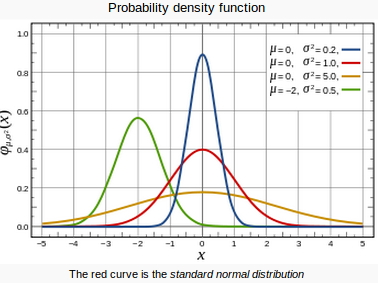
\includegraphics[scale=0.6]{./Pictures/rbf.jpg}
\caption{径向基核函数曲线分布示意图}
\label{rbf}
\end{figure}


而不同类型的故障需要不同核参数使得其检测效果最佳,在本章中考虑选择一系列的核参数建立对应的模型,利用相同的训练数据训练这些模型,再将这些模型的检测效果利用贝叶斯推论转化为概率的形式集成起来,从而实现了对不同类型的故障均有有较好的检测效果,同时,也避免了核参数选择的问题。因此,这一系列的核参数的范围必须有足够的广度,能够适用于不同类型的故障,我们选择了如下的B组参数:
\begin{equation}
c_i=2^{(i-1)}\times5m ~~~~\quad i=1,\ldots,B.
\end{equation}
$m$表示训练数据的维数,$B$表示模型的数目,当$B$选择恰当时候核参数具有比较大的范围,能够较好的满足不同类型的故障的需求。因此,不同核参数的模型对应的核矩阵特征分解可表示为:
\begin{equation}\label{}
\textbf{K}^{(i)}=\textbf{E}^{(i)}\Lambda^{(i)}\textbf{E}^{(i)T}.
\end{equation}
其相对应的检测结果可表示为:
\begin{equation}\label{}
\textbf{T}^{(i)}=\textbf{K}^{(i)}\textbf{E}^{(i)}.
\end{equation}
再通过$T^2$和SPE可以利用每一个子模型对新的样本数据$\textbf{x}$进行检测,然后通过贝叶斯推论将其转化为故障概率的形式:
\begin{equation}\label{18}
P^{(i)}_{T^2}(F|\textbf{x})=\frac{P^{(i)}_{T^2}(\textbf{x}|F)P^{(i)}_{T^2}(F)}{P^{(i)}_{T^2}(\textbf{x})},
\end{equation}
\begin{equation}\label{19}
P^{(i)}_{SPE}(F|\textbf{x})=\frac{P^{(i)}_{SPE}(\textbf{x}|F)P^{(i)}_{SPE}(F)}{P^{(i)}_{SPE}(\textbf{x})},
\end{equation}
分母中的 $P^{(i)}_{T^2}(\textbf{x})$ 和 $P^{(i)}_{SPE}(\textbf{x})$ 可以通过全概率进行计算:
\begin{equation}\label{}
P^{(i)}_{T^2}(\textbf{x})=P^{(i)}_{T^2}(\textbf{x}|N) P^{(i)}_{T^2}(N)+P^{(i)}_{T^2}(\textbf{x}|F)P^{(i)}_{T^2}(F),
\end{equation}
\begin{equation}\label{}
P^{(i)}_{SPE}(\textbf{x})=P^{(i)}_{SPE}(\textbf{x}|N) P^{(i)}_{SPE}(N)+P^{(i)}_{SPE}(\textbf{x}|F) P^{(i)}_{SPE}(F),
\end{equation}
其中 $N$ 和 $F$ 分别代表了正常和故障情况,
$p(N)$ 和 $p(F)$ 是正常和故障情况下的先验概率。
当显著水平设为 $\alpha$,
$p(N)$ 的值此时就是 $\alpha$, $p(F)$ 的值则是为 $1-\alpha$。
为了计算故障概率的大小,条件概率$P^{(i)}_{T^2}(\textbf{x}|N)$,
$P^{(i)}_{T^2}(\textbf{x}|F)$, $P^{(i)}_{SPE}(\textbf{x}|N)$,
和 $P^{(i)}_{SPE}(\textbf{x}|F)$
被定义为如下的形式:
\begin{equation}\label{}
P^{(i)}_{T^2}(\textbf{x}|N)=exp(-T^{2(i)}/T^{2(i)}_{limit}),
\end{equation}
\begin{equation}\label{}
P^{(i)}_{SPE}(\textbf{x}|N)=exp(-SPE^{(i)}/SPE^{(i)}_{limit}),
\end{equation}
\begin{equation}\label{}
P^{(i)}_{T^2}(\textbf{x}|F)=exp(-T^{2(i)}_{limit}/T^{2(i)}),
\end{equation}
\begin{equation}\label{25}
P^{(i)}_{SPE}(\textbf{x}|F)=exp(-SPE^{(i)}_{limit}/SPE^{(i)}),
\end{equation}
上式中的 $T^{2(i)}_{limit}$ 和 $SPE^{(i)}_{limit}$ 分别代表第 $i$ 个模型的控制限。
通过权重组合的方式可以将故障的概率指标表示为如下形式:
\begin{equation}\label{26}
ET^2_{new}=\sum_{i=1}^{n_s}\frac{P^{2(i)}_{T^2}(F|\textbf{x})}{\sum_{j=1}^{n_s}P^{(j)}_{T^2}(F|\textbf{x})},
\end{equation}
\begin{equation}\label{27}
ESPE_{new}=\sum_{i=1}^{n_s}\frac{P^{2(i)}_{SPE}(F|\textbf{x})}{\sum_{j=1}^{n_s}P^{(j)}_{SPE}(F|\textbf{x})}.
\end{equation}
此时,显著水平$\alpha$扮演了控制限的作用,当$ET^2_{new}\prec\alpha$和$ESPE_{new}\prec\alpha$时候,认为系统处于正常工况状态,当$ET^2_{new}\succ \alpha$ 或者$ESPE_{new}\succ\alpha$的时候,则认为系统有检测到故障。
\section{过程监测策略}
我们将上一节所介绍的方法称为EKECA,利用EKECA实现故障检测的具体流程可以分为离线建模和在线监测两部分,该算法的流程图如图\ref{flowchart}所示,而具体实现为:
\begin{figure}[htb]
\centering
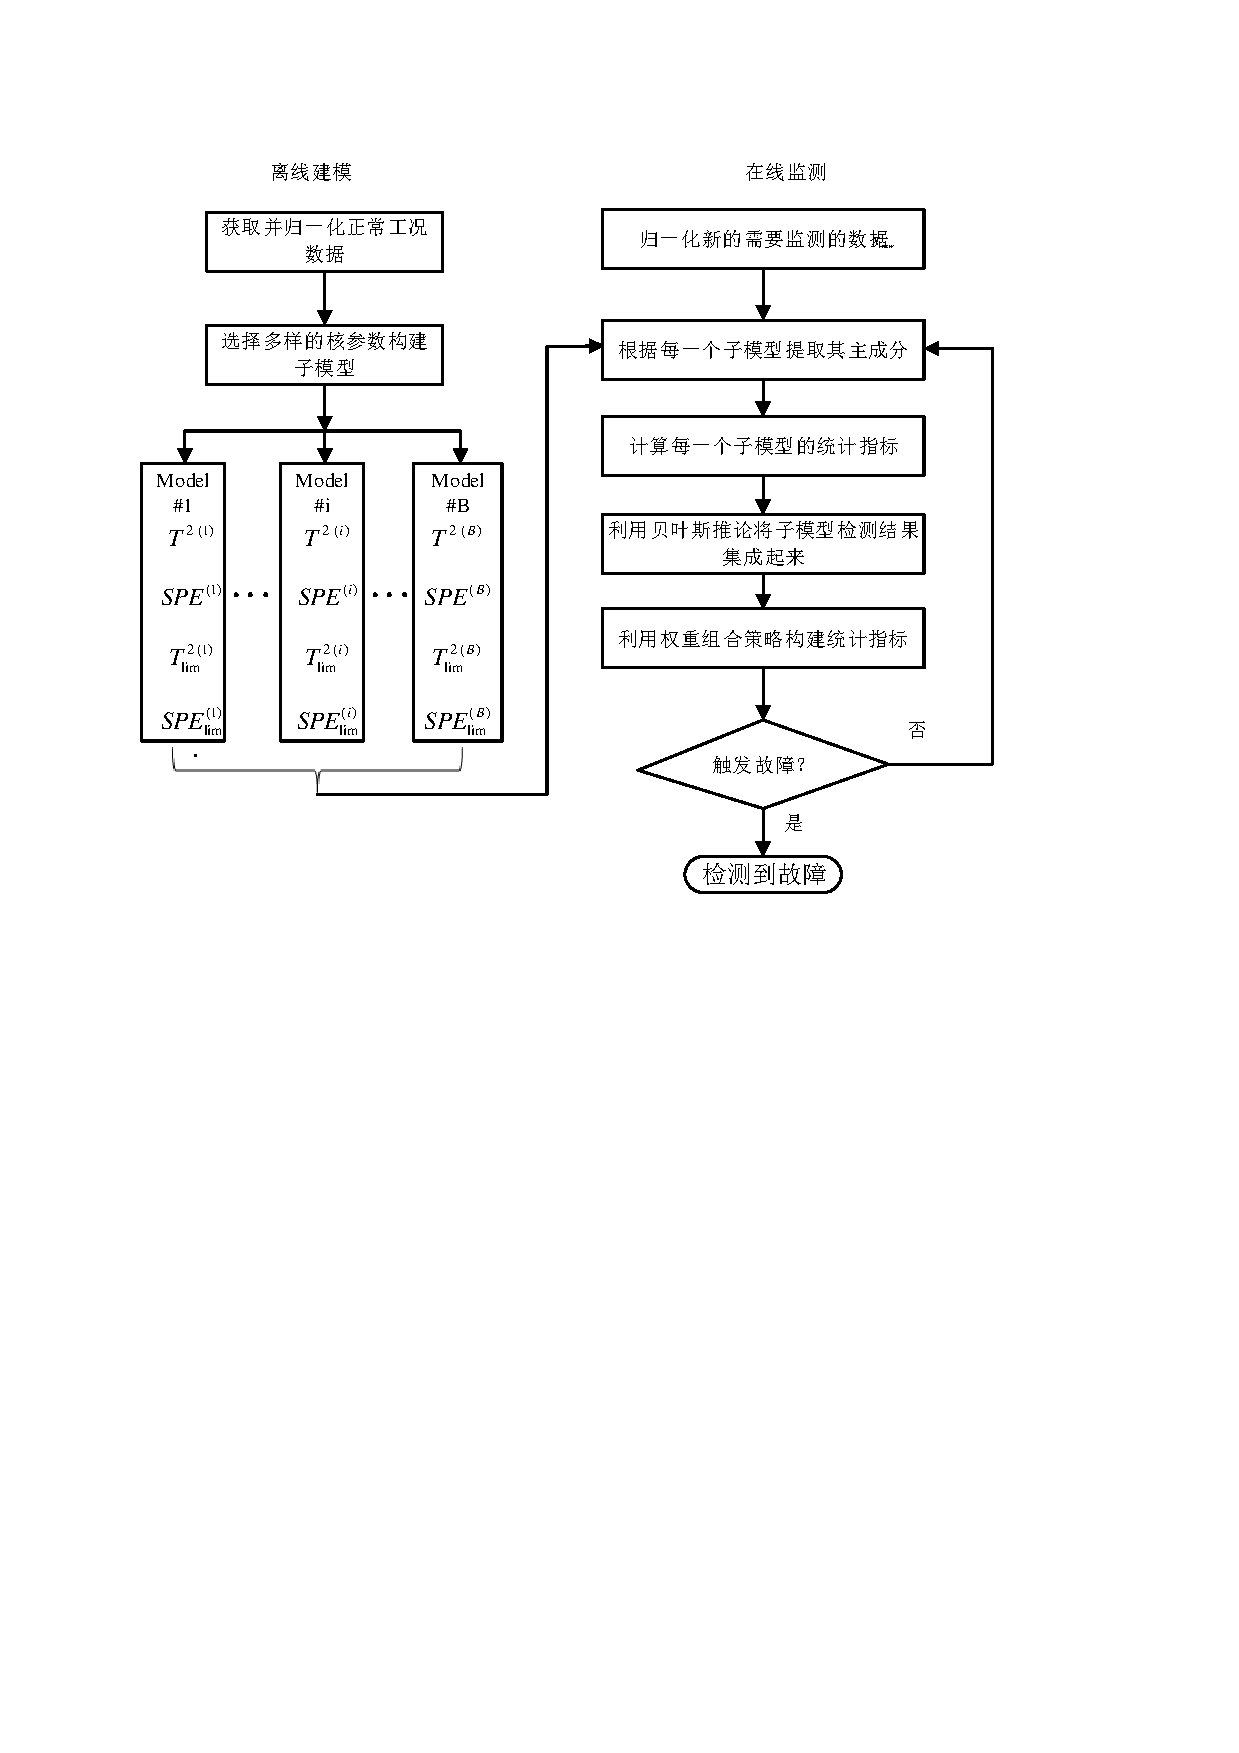
\includegraphics{./Pictures/flowchart.pdf}
\caption{EKECA算法流程图}
\label{flowchart}
\end{figure}

离线建模:

$(1)$ 采集正常工况状态下的生产数据,经过标准化之后作为训练集 $\textbf{X}$ ;

$(2)$ 针对每一个核函数,构造KECA模型并通过$\|\textbf{e}_i\|^2=1/(N\lambda_i)$归一化其负载矩阵$\textbf{E}$;

$(3)$ 通过 $\textbf{T}^{(i)}=\textbf{K}\textbf{E}^{(i)}$提取每一个子模型中的主成分信息;

$(4)$ 计算每一个子模型中的统计指标$T^2$和SPE以及相对应的控制限。

在线监测:

$(1)$ 采用与离线阶段相同的方法归一化在线数据 $\textbf{x}_{new}$ ;

$(2)$ 通过$\textbf{t}^{(i)}_{k}=\textbf{K}_{new}^{(i)}\textbf{e}^{(i)}_{k} , k=1,...,p^{(i)}$提取 $\textbf{x}_{new}$ 的主成分部分;

$(3)$ 将每一个子模型的检测效果通过贝叶斯推论转化成概率的形式并将他们集成起来;

$(4)$ 判断是否有故障发生,其中 $ET^2_{new}\prec\alpha$ 并且 $ESPE_{new}\prec\alpha$ 过程处于正常状态,而 $ET^2_{new}\succ\alpha$ 或者 $ESPE_{new}\succ\alpha$ 则代表检测到了故障。



\section{TE过程仿真研究}


\section{插入算法伪代码}
以下是插入算法伪代码示例,如算法\ref{alg:skeleton_dt}所示。

\begin{algorithm}[!htb]
\caption{基于距离变换的骨架提取}
\label{alg:skeleton_dt}
\begin{algorithmic}[1]
\Require 前景的二值图 bw \Comment{像素的灰度值为0或1} 
\Ensure 骨架图 skel
\State // 第1次遍历:从上往下,从左往右
\For{$i=1,\dots ,M$} \Comment{M是二值图的高度}
    \For{$j=1,\dots ,N$} \Comment{N是二值图的宽度}
        \State bw[i][j] = 1 + min(bw[i][j-1], bw[i-1][j])  \Comment{min函数取极小值} 
    \EndFor
\EndFor
\State // 第2次遍历:从下往上,从右往左
\For{$i=M,\dots ,1$}
    \For{$j=N,\dots ,1$}
        \State bw[i][j] = 1 + min(bw[i][j], bw[i+1][j], bw[i][j+1])
    \EndFor
\EndFor
\State // 第3次遍历:获取骨架图
\State skel 的空间分配,并将每个像素初始化为0
\For{$i=1,\dots ,M$}
    \For{$j=1,\dots ,N$}
        \State t = max(bw[i-1][j], bw[i+1][j], bw[i][j-1], bw[i][j+1])  \Comment{max函数取极大值} 
        \State t = max(t, bw[i-1][j-1],bw[i-1][j+1],bw[i+1][j-1],bw[i+1][j+1])
        \If {bw[i][j]>=t}
        	\State skel[i][j]=1 \Comment{骨架点} 
        \Else 
        	\State skel[i][j]=0
        \EndIf
    \EndFor
\EndFor
\end{algorithmic}
\end{algorithm}

\section{插入源代码}
代码示例:

\begin{lstlisting}[language=C] 
int main(int argc, char ** argv) 
{ 
	printf("Hello world! \n"); 
	return 0; 
} 
\end{lstlisting} 

\section{插入定义、定理等}
实例来自 https://github.com/eclipselu/zjuthesis-mphil。

\begin{hypo}
待月西厢下,迎风户半开;隔墙花影动,疑是玉人来。
\begin{eqnarray}
  \label{eq:eqnxmp}
  c & = & a^2 - b^2\\
    & = & (a+b)(a-b)
\end{eqnarray}
\end{hypo}

\begin{defin}
子曰:「道千乘之国,敬事而信,节用而爱人,使民以时。」
\end{defin}

\begin{theo}
犯我强汉者,虽远必诛。\hfill —— 陈汤(汉)
\end{theo}

\begin{pro}
天不言自高,水不言自流。
\begin{gather*}
\begin{split} 
\varphi(x,z)
&=z-\gamma_{10}x-\gamma_{mn}x^mz^n\\
&=z-Mr^{-1}x-Mr^{-(m+n)}x^mz^n
\end{split}\\[6pt]
\begin{align} \zeta^0&=(\xi^0)^2,\\
\zeta^1 &=\xi^0\xi^1,\\
\zeta^2 &=(\xi^1)^2,
\end{align}
\end{gather*}
\end{pro}



\chapter{基于MVU\_KECA的非线性故障检测}
\noindent \textbf{摘要}
\quad 针对工业过程中的非线性检测问题,一种常用的解决方法是引入核函数,利用核函数实现对原始数据进行高维映射,从而将非线性问题近似线性化。
然而,到目前为止,关于核函数中参数选择问题没有统一的结论。
本章将最大方差展开(MVU)引入到核熵成分分析(KECA),利用MVU学习得到核矩阵,提出了一种基于KECA\_MVU的非线性故障检测方法。
其主要思想是在利用KECA实现检测过程中,其核矩阵由原来的直接通过核函数计算替换为通过MVU 解优化得到,再通过线性回归近似得到原始数据到降维输出的非线性映射,最后利用该映射实现在线检测,从而避免了核参数选择的盲目性。
此外,该方法也继承了MVU 的特性,能够在降维后实现数据分布边界的保持。
在TE 过程的仿真结果也验证了该方法能够有效地实现对故障的检测。\\
\textbf{关键词}\quad 故障检测;非线性;MVU;线性回归;KECA

\section{引言}
现代工业工程中引入了集散控制系统(DCS),利用DCS可以有效地对工业过程实现集中管理和分散控制。
DCS大大的方便了数据的采集,
然而,采集到的数据由于工业过程中约束条件以及平衡的存在使得数据具有高相关性、高维度、非高斯性等特点。
而实际的工业过程中的数据波动可以通过少量的变量就能够进行有效的解释,
这就使得这一类通过将高维数据映射到低维而实现提取其主成分的数据处理方法变得流行起来。
通过降维将数据分为互补的两个部分:系统部分和残差部分,
这两部分分别可以用来反映降维模型内部的波动和模型外部的波动,
从而实现了对生产过程的监测。
核方法是一种被广泛用来处理非线性降维的方法,
该方法有效地通过核矩阵的空间映射将原始数据的非线性分布近似线性化。
KECA就是一种从信息熵角度出发的利用核函数实现非线性数据处理的方法,其具有较好的监测效果。
但是,KECA并没有考虑到数据的边界分布特性,
在实际的生产数据中,能够表征其特性的过程数据实际是一个低维结构,而其原始数据结构则是高维度的结构,
也就是说反映数据波动特性的成分是嵌入高维空间的低维结构。
使用KECA对数据进行降维,并不能很好地从数据结构的角度来解释边界分布这个问题。
此外,如何确定KECA中核函数的最优和参数也没有固定的结论。
流行学习是近年来广泛被研究的一类有效地处理非线性数据降维的方法,
它们通过在局部和全局分别进行线性和非线性的数据分布假设,揭示了非线性数据的内在规律,
然后引入优化求解得到能够保持数据最优分布特征的低维嵌入表示。
最大方差展开(MVU)是比较有代表性的一种流行学习方法,
其假设条件是数据在局部满足线性条件,并且在降维前后局部范围k-邻近点之间的欧氏距离保持不变。
因此,其目标可以转换为最大化低维数据的邻近点的欧式距离,
这一点与PCA的目标一致,即其目标是通过保持低维数据方差最大实现降维,
再通过引入核函数,
该方法将训练数据的核矩阵求解问题转换为求解一个半定规划问题,
该问题的最优解即为所求核矩阵$K$。
MVU基于几何分布的流形假设可以使得该方法很好地保存数据分布的边界,
而故障检测离线建模阶段就是通过离线数据建立模型从而确定生产过程的波动边界,
这说明MVU可以很好地用于过程监测。
然而,MVU通过半定规划得到核矩阵并没有显示的数据映射表达式,
故不能直接应用于过程监测。
邵纪东和姚远等人分别提出了使用线性回归和搞死过程模型来得到投影矩阵,
从而解决了MVU在用于过程监测时候实现在线监测的问题。

本章提出了一种基于核熵成分分析和最大方差展开的新的降维方法(KECA\_MVU),
并将其用于故障检测。
该方法在离线建模阶段利用MVU学习得到核矩阵,
再通过选择熵最大的方向将数据降维得到其得分向量,
然后利用线性回归得到原始数据到降维表示的最优线性近似投影,
最后利用该投影实现在线检测。

\section{最大方差展开}
%
%近年来,流形广泛地用于机器学习领域,并逐步地应用于过程监当中。
%流形(Manifold)是局部具有欧式空间性质的空间,它可以视为对线性子空间的非线性推广,
%其思想是假设数据点分布在嵌入于外围欧式空间当中的流形结构上。
%MVU是通过保持局部距离来实现嵌入的展开。
%\subsection{MVU回顾}

MVU与PCA有着相同的优化目标,是PCA的非线性扩展。
其优化目标是使降维空间中相邻点之间的欧式距离最大,
该目标可以转化为使得映射后的方差最大从而实现数据降维,
它本质上是一种特殊的Kernel PCA。
在使用KPCA降维过程中,通过寻找特定的核函数将数据数据投影到高维的特征空间当中去,
而在数据投影过程中可以计算得到核矩阵$\textbf{K}$。
MVU则是通过直接利用训练数据定义核矩阵实现了将输入数据的流形结构展开到核特征空间过程当中的目标,
定义过程可以转换为一个半正定规划(SDP)问题,
对SDP求最优解即得到了核矩阵$\textbf{K}$。
由于SDP求解是一个凸优化问题,从而确保了所获得的核矩阵是全局最优。
设训练数据为$\textbf{x}_i, \ldots, \textbf{x}_n$,$\textbf{x}_n ~ \epsilon~\textbf{R}^D$,
将其映射到核特征空间$\mathcal{F}$当中,映射后的数据表示为\bm{$\Phi(\textbf{x}_i)$}, \ldots, \bm{$\Phi(\textbf{x}_n)$},
设$\textbf{y}_i, \ldots, \textbf{y}_n$ ,$\textbf{y}_n ~ \epsilon~\textbf{R}^d$,是其降维后的嵌入表示。
其中,$N$代表样本数量,$D$代表输入数据的变量数,$d$代表降维后低维嵌入的维数,且满足$d < D$。
MVU通过映射\bm{$\Phi$}既实现了展开输入数据的流形结构,又保证了输入数据与输出的低维嵌入数据是局部等距的,
设其局部临近点为$k$。
因此,为了展开流形结构,MVU的优化目标就可以表示为使得输出的低维嵌入结构中点的欧式距离最大:

\begin{equation}
\label{MVU}
\Gamma= \frac{1}{2N}\sum_{i=1}^{N}\sum_{j=1}^{N}\parallel\Phi(\textbf{x}_i)-\Phi( \textbf{x}_j)\parallel^2
\end{equation}

为了使得式(\ref{MVU})所表示的值最大,需要满足以下几条约束条件:

\textrm{I}\quad 局部等距性:\\
该约束是用来保证核空间当中的局部流形结构。
设$\mathbf{W}~\epsilon ~\textbf{R}^{N\times N}$ 是二值邻接矩阵,
可以用其值来判断$\textbf{x}_i$和$\textbf{x}_j$是否在$k$近邻区域内相邻。
因此,如果$\textbf{x}_i$和$\textbf{x}_j$相邻,有$\mathbf{W}_{ij}=1$,
或者$\textbf{x}_i$与$\textbf{x}_j$与另一个点的同时相邻,有$[\mathbf{W}^T\mathbf{W}]_{ij}=1$。
局部等距约束条件就可以表示为:
\begin{equation}
\label{iso}
\|\bm{\Phi(\textbf{x}_i)}-\bm{\Phi(\textbf{x}_j)}\|^2=\|\textbf{x}_i-\textbf{x}_j\|^2
\end{equation}

\textrm{II}\quad 中心化:\\
中心化约束条件的作用是用来消除数据在映射过程中由于旋转和平移等操作所产生的自由度,
可以将其表示为:
\begin{equation}
\label{center}
\sum_{i=1}^{N}\bm{\Phi(\textbf{x}_i)}=0
\end{equation}

从公式(\ref{MVU})\~(\ref{center})可知,式中存在利用等式约束条件对欧式距离的二次方求解最优值,
该过程并不能保证所得结果是全局最优。
为了保证所得最优解为全局最优,对输出低维嵌入空间定义内积矩阵,
$\mathbf{K}_{ij}=\bm{\Phi}(\mathbf{x}_i)^T\bm{\Phi}(\mathbf{x}_j)$,
公式(\ref{iso})的等距性约束以可以由展开为:
\begin{equation}
%\label{iso}
\|\bm{\Phi(\textbf{x}_i)}-\bm{\Phi(\textbf{x}_j)}\|^2=\|\textbf{x}_i-\textbf{x}_j\|^2
=\mathbf{K}_{ii}+\mathbf{K}_{jj}-2\mathbf{K}_{ij}
\end{equation}

将内积带入到目标函数\ref{MVU}和中心化约束\ref{center},
优化目标可以表示为:
\begin{equation}
\label{obj}
\Gamma= \frac{1}{2N}\sum_{i=1}^{N}\sum_{j=1}^{N}\parallel\bm{\Phi}(\textbf{x}_i)-
\bm{\Phi}( \textbf{x}_j)\parallel^2
=\frac{1}{2N}\sum_{i=1}^{N}\sum_{j=1}^{N}(\mathbf{K}_{ii}+\mathbf{K}_{jj}-2\mathbf{K}_{ij})
\end{equation}

同理,公式\ref{center}可以利用内积的形式展开为:
\begin{equation}
\label{center_new}
\|\sum_{i=1}^{N}\bm{\Phi(\textbf{x}_i)}\|^2
=\sum_{i=1}^{N}\sum_{j=1}^{N}\bm{\Phi}(\textbf{x}_i)^T\bm{\Phi}(\textbf{x}_j)
=0
\end{equation}

再将公式(\ref{center_new})带回到公式(\ref{obj})中,
优化目标可以表示为:
\begin{equation}
%\label{obj_2}
\Gamma= \frac{1}{2N}\sum_{i=1}^{N}\sum_{j=1}^{N}(\mathbf{K}_{ii}+\mathbf{K}_{jj}-2\mathbf{K}_{ij})
      = Tr(\mathbf{K})
\end{equation}

此时,最优解问题转化为求解核矩阵$\mathbf{K}$的迹,为了保证该过程为一个凸优化过程,
需要在上面等式约束的基础上附加一不等式约束条件$\mathbf{K}\succeq 0$,
也就是要求核矩阵满足半正定条件。
这样,求解MVU最优解的过程就变成了一个半正定规划(SDP)问题,其具体形式为:
%\begin{equation}
%\label{obj_final}
%\mathrm{max}\quad Tr(\mathbf{K})\\
%s.t. \quad \mathbf{K}\succeq 0\\
%     \quad \sum_{ij}\mathbf{K}_{ij}=0\\
%     \mathbf{K}_{ii}+\mathbf{K}_{jj}-2\mathbf{K}_{ij}=\|\textbf{x}_i-\textbf{x}_j\|^2,
%\mathbf{W}_{ij}=1|[\mathbf{W}^T\mathbf{W}]_{ij}=1
%\end{equation}
%\begin{gather}
%\mathrm{max}\quad Tr(\mathbf{K})\quad\quad\quad\quad s.t. \quad \mathbf{K}\succeq 0 \notag \\
%\quad\quad\quad\quad \quad\quad\quad\quad\quad\quad\quad\quad\quad~~\sum_{ij}\mathbf{K}_{ij}=0 \notag \\
%\quad\quad\quad\quad\quad\quad\quad\quad\quad\quad\quad\quad \mathbf{K}_{ii}+\mathbf{K}_{jj}-2\mathbf{K}_{ij}
%=\|\textbf{x}_i-\textbf{x}_j\|^2
%\end{gather}
\begin{equation}
\label{obj_final}
\begin{split}
\mathrm{max}\quad Tr(\mathbf{K}) \quad\quad s.t.\quad& \mathbf{K}\succeq 0  \\
& \sum_{ij}\mathbf{K}_{ij}=0  \\
&\mathbf{K}_{ii}+\mathbf{K}_{jj}-2\mathbf{K}_{ij}
=\|\textbf{x}_i-\textbf{x}_j\|^2 \\
\end{split}
\end{equation}
其中,对于所有$(i,j)$有$\mathbf{W}_{ij}=1$或者$[\mathbf{W}^T\mathbf{W}]_{ij}=1$。
以上凸优化有多种解法,本文中对该凸优化求解可以利用工具包CSDP实现,
其具体介绍可以参考相应的文章。

通过公式(\ref{obj_final})可以得到MVU的最优解$\mathbf{K}$,
再对内积核矩阵$\mathbf{K}$进行特征分解,可以得到输出$\mathbf{y}_i$的表达形式。
设$V_{\alpha i}$表示特征值$\lambda_{\alpha}$对应的第$\alpha$个特征向量的第$i$ 个元素,
则核矩阵可以表示为:
\begin{equation}
\label{diag}
\mathbf{K}_{ij}=\sum_{\alpha=1}^{d}\lambda_{\alpha}\mathbf{V}_{\alpha i}\mathbf{V}_{\alpha j}
\end{equation}
公式中的$d$表示低维嵌入的维数,
该嵌入结构与输入$\mathbf{x}_{i}$是局部$k$邻接等距的,
它可以通过输出的第$\alpha$个元素表示:
\begin{equation}
\label{output}
\mathbf{Y}_{\alpha i}=\sqrt{\lambda_{\alpha}V_{\alpha i}}
\end{equation}
由此,该局部等距的低维嵌入结构就通过谱分解被表示出来了。

\section{KECA\_MVU}

从上一节的分析可知,MVU的目标函数依旧是获得方差最大的方向,它是PCA的一种非线性扩展。
MVU通过求解SDP问题得到全局最优解$\mathbf{K}$,
再利用谱分解由特征值和特征向量组合得到了降维后的低维嵌入的表示。
本章则是信息熵的角度出发,将利用SDP所获得的核矩阵$\mathbf{K}$不再按照特征值的大小进行排序,
而是根据瑞利熵的大小进行排序获取其投影方向,然后对非线性数据实现降维。
结合上一章所介绍的知识,在特征空间当中利用MVU进行数据投影时,
将$\bm{\Phi}$投影到第$i$个主成分$\mathbf{u}_i$可以表示为:
\begin{equation}
P_{\mathbf{u}_i}\bm{\Phi}=\sqrt{\lambda_i}\mathbf{e}_i^T ,
\end{equation}
其中,$\lambda_i$和$\mathbf{e}_i$分别表示特征值以及与之对应的的特征向量。
而其瑞利熵的估计可以表示为:
\begin{equation}
\label{entropy_estimate}
\hat{V}(p)=\frac{1}{N^2}\sum \limits_{i=1}^{N}(\sqrt\lambda_i \mathbf{e}_i^T\textbf{1})^2.
\end{equation}%\newline
这就不难发现瑞利熵的估计是由所有到MVU主成分方向上的投影组成的。
而只有当对应主成分轴的$\lambda_i\neq 0$并且$\mathbf{e}_i^T\mathbf{1}\neq 0$才能够使得其对瑞利熵的估计值有贡献。
而那些对瑞利熵贡献较大的主成分方向包含了大部分关于由输入数据提供的概率密度函数的形状信息,
如果仅仅是通过选择最大的前$d$个特征值,
那么从信息熵的角度来看对数据进行投影时候其投影方向可能有并不包含信息的特征向量。

设$U_d$是KECA\_MVU的数据投影方向,由前面的分析可知,
$U_d$是由MVU投影当中对瑞利熵贡献最大的前$d$个特征向量张成的子空间。
为了使得数据投影后能够保存尽可能多的输入数据的信息,
则KECA\_MVU的优化目标可以表示为:
\begin{equation}
\label{obj_MVU}
\min \limits_{\lambda_1,e_1,\ldots,\lambda_N,e_N} \quad \hat{V}(p)-\hat{V}_{d}(p)
\end{equation}
其解可以表示为:
\begin{equation}
\label{projection}
\bm{\Phi}_{eca}=P_{U_d}\bm{\Phi}=\bm{\Lambda}_d^{\frac{1}{2}}\mathbf{E}_{d}^T,
\end{equation}
其中,$\bm{\Lambda}_d$和$\mathbf{E}_{d}$分别表示MVU求解得到的核矩阵特征分解之后对应的特征值和特征向量矩阵。
而与$\bm{\Phi}_{eca}$对应的瑞利熵的估计可以表示为:
\begin{equation}
\label{d_estimate}
V_d(p)=\frac{1}{N^2}\mathbf{1}^T\mathbf{E}_{d}\bm{\Lambda}_d\mathbf{E}_{d}^T\mathbf{1}
=\frac{1}{N^2}\mathbf{1}^T\mathbf{K}_{eca}\mathbf{1}
\end{equation}
将公式(\ref{d_estimate})带入到公式(\ref{obj_MVU})当中,KECA\_MVU的优化目标可以表示为:
\begin{equation}
%\label{obj_MVU_final}
\min \limits_{\lambda_1,e_1,\ldots,\lambda_N,e_N} \quad 
\frac{1}{N^2}\mathbf{1}^T(\mathbf{K}-\mathbf{K}_{eca})\mathbf{1}
=\frac{1}{N^2}\sum_{j=d+1}^{N}\psi_j
\end{equation}
公式当中的$\psi_j$则与公式(\ref{entropy_estimate})中的$j$最大项相关,
也就是通过选择前$d$项最大的瑞利熵的值可以实现数据投影后保留的信息最多,
KECA\_MVU通过选择瑞利熵最大的前$d$项作为数据投影的方向实现了数据的有效降维。
%投影P



\chapter{一些反馈的问题}

以下将对一些在这个模版发布两年间,
使用的各位网友发给我邮件询问相关问题的内容的解答作一个集中记录。
其中的一些问题及我提供的解决方案可以供广大有不同需要的网友们参考。

\section{关于使用author year 参考文献引用方式的问题}

这是我收到的第一封回复邮件,
问题相对比较简单,
是一个叫Jerry Chen的网友提给我的,
这个模版默认是使用数字编号对标示参考文献引用的,
Jerry Chen 网友希望使用author year这种格式进行参考文献的标注。
就像如下的格式。

\begin{center}
\begin{tabular}{p{3cm}cp{5cm}}
$\backslash$citet\{jon90\} & --> & Jones et al. (1990) \\
\end{tabular}
\end{center}

要实现这个显示校果,需要对ZJUthesis.cls文件以及ZJUthesis.bst文件进行修改,
其中对ZJUthesis.bst文件修改可以通过修改dbjfile\_wdj\_V1.0.dbj文件的方式进行修改。
分别如下:

\begin{itemize}
\item{ZJUthesis.cls文件中}

第41行是关于正文中参考文献引用标记格式设置的。
把它由数字排序方式变为作者年代的排序方式,即
由:

{
\zihao{-5}
\verb+\RequirePackage[sort&compress,longnamesfirst,square,super]{natbib}+
}

修改为:

{
\zihao{-5}
\verb+\RequirePackage[longnamesfirst,round,authoryear]{natbib}+
}

第654行是关于正文后参考文献列表的结构格式,
将其由数字标号方式改为作者年代标记方式。
即由:

{
\zihao{-5}
\verb+\setcitestyle{numbers, round, comma, aysep={}, yysep={,}, notesep={,}}+
}

修改为:

{
\zihao{-5}
\verb+\setcitestyle{authoryear, round, comma, aysep={}, yysep={,}, notesep={,}}+
}

\item{dbjfile\_wdj\_v1.0.dbj文件中}

对选项
\%STYLE OF CITATIONS: 
修改为:  ay

对选项
\%MAX AUTHORS BEFORE ET AL: (if regular cite not selected)
修改为:  mct-1,\%: One et al

\end{itemize}

然后再生成新的ZJUthesis.bst文件即可,该文件的生成方式见第五章内容中介绍。

\section{关于chapter居中格式的问题}

这个模版中,每一章的标题默认是左对齐设置的,
当然有的同学想设置成居中,比如给我发邮件的dongliang同学。这个也很简单,
只要修改ZJUthesis.cls文件中的第546行,
由:

{
\zihao{-5}
\verb+\CTEXsetup[format={\noindent}]{chapter}+
}

修改为:

{
\zihao{-5}
\verb+\CTEXsetup[format={\centering}]{chapter}+
}

即可,关于该处设置的含义可以参考CTeX自带的帮助文档ctex.pdf。

\section{关于章级目录有时居中有时不居中的解决方案}

这个问题有点儿类似上面的情况,
要求更复杂一些,是由叫zwb的网友提给我的。
但这个问题的解决方案更简单,只要在需要居中的章节前加上

{
\zihao{-5}
\verb+\CTEXsetup[format={\centering}]{chapter}+
}

在需要左对齐的章名前加上

{
\zihao{-5}
\verb+\CTEXsetup[format={\noindent}]{chapter}+
}

即可。


\section{关于标题两行还写不下的问题}

这是一个叫FRW的同学提给我的,Ta的标题太长,
我的模版里只设置了两行写标题,需要第三行,
这就需要修改ZJUthesis.cls文件来适应这个问题了。
其实跟添加第二行的方式一样,只是增加了一个第三行内容的命令及
与第二行相同的判断。

首先增加两个命令
$\backslash$EtitleB 和 $\backslash$englishtitleB,
再对这两个命令的使用位置进行定义。

这两个命令的定义语句如下:

{\zihao{-5}
\verb+\newcommand\EtitletB[1]{\def\ZJU@value@EtitletB{#1}}+

\verb+\newcommand\englishtitletB[1]{\def\ZJU@value@englishtitletB{#1}}+
}

在两处对标题多行判断的后面加上这样几句:

\begin{itemize}
\item{在首页上的题目部分}

{
\zihao{-5}
\begin{verbatim}
        \fi\\[3mm]
        % 第三行英文标题
        &
        \ifx\ZJU@value@EtitletB\undefined
	  \hfil
	\else
	  {\bfseries\zihao{-2}\ZJUunderline[260pt]{\ZJU@value@EtitletB}}
        \fi\\
\end{verbatim}
}
第一行的\verb+\fi\\[3mm]+意思是从这个\verb+\\fi\\+处后面开始加代码,
这个3mm是为了每一行高度都一样设置,这个从上面第一行最后一句就可以看出来。
增加代码中的“\&”符号是因为这个地方用的是tabular环境用于对齐。

\item{在英文标题页的部分}

{
\zihao{-5}
\begin{verbatim}
% 判断英文标题有无第三行
      \ifx\ZJU@value@englishtitletB\undefined
        \hfil
      \else
        \ZJUunderline[300pt]{\ZJU@value@englishtitletB}
      \fi}
\end{verbatim}
}

增加的代码与上面一条类似,不再多述。

\end{itemize}


\section{目录层次与子目录分层缩进}

FRW同学还提出了另一个问题,
这个模版的目录中只有两层标题,想要三层标题,
而且这个模版中目录两层标题的字体字号都一样,
想要不同层次有不同缩进。
这个问题也容易解决,都在ZJUthesis.cls中有相应命令设置。
第601至第620行是关于目录的格式设置,
比如增加及修改下面的所列,就可以满足上面的要求。

{
\zihao{-5}
\begin{verbatim}
  \renewcommand{\cftsecpagefont}{\rm\zihao{-4}}
  \renewcommand{\cftsubsecleader}{\cftdotfill{\cftdot}}
  \renewcommand{\cftsubsecfont}{\fangsong\zihao{-4}}
  \renewcommand{\cftsubsecdotsep}{\cftdotsep}
  \renewcommand{\cftsubsecpagefont}{\rm\zihao{-4}}
  \setlength{\cftbeforechapskip}{-2pt}
  \setlength{\cftbeforesecskip}{-2pt}
  \setlength{\cftbeforesubsecskip}{-2pt}
  \setlength{\cftsecindent}{2eM}
  \setlength{\cftsubsecindent}{4eM}
  \setcounter{tocdepth}{2}
\end{verbatim}
}

这几句增加了subsection一级的目录显示格式,
把section及subsecion目录列表前面的缩进设置为2个字符和4个字符,
最后又把目录的显示深度由原来的1设置为2,就可以显示三级标题了。

\section{关于分章参考文献的用法}

这个模版里头的参考文献是一个章节格式的,
全文只有一个参考文献章,这是一个一般的情况。
当然有的同学希望能采用每一章都有自己参考文献的解决方案。
这个方案也比较简单,只用修改如下几个地方。

\begin{enumerate}
\item{使用chapterbib包}

首先在导言区,加入chapterbib包,带上sectionbib选项。

\item{每章增加参考文献命令}

这个模版的源文件每一章都是一个甚至多个独立的tex文件,
并在主文件“论文模版示例.tex”中用“include”命令
\footnote{这个地方要注意不要使用“input”命令,使用这个命令不能实现分章参考文献}
将其包含在主文件中。
要在每章的tex文件的最后,加上
\verb+\ZJUthesisbib{thesisbib}+
这一条命令,假如是把所有章的参考文献数据库都写在一个文件里,
比如这个模版中的thesisbib.bib,
那这个命令的参数在所有章中都是“thesisbib”。
如果每章的参考文献数据库都有各自的独立的数据库文件,
那么每章中这个命令的参数就不同。

\item{删去原来的参考文献引用命令}

把全篇最后的参考文献引用命令删去,用不到了。

\item{修改编译命令}

原来生成PDF文件时,bibtex运行是一条命令“bibtex 论文模版示例”,
现在就要根据有几章有参考文献列几条不同的bibtex命令了。
即:

{
\zihao{5}
\begin{verbatim}
bibtex .\Chapter\chap1
bibtex .\Chapter\chap2
bibtex .\Chapter\chap3
bibtex .\Chapter\chap4
bibtex .\Chapter\chap5
bibtex .\Chapter\chap6
\end{verbatim}
}

\end{enumerate}

\section{第X章格式的修改}

这个模版的每一章的章节号直接是阿拉伯数字,
有同学想用第X章这种格式,
修改也很简单,根据CTeX自带的帮助文档ctex.pdf,
只要将ZJUthesis.cls中的第492行由

{
\zihao{5}
\verb+\CTEXsetup[name={,}]{chapter}+
}

修改为:

{
\zihao{5}
\verb+\CTEXsetup[name={第,章}]{chapter}+
}

即可。
至于字体修改,居中还是偏左,都是在这几行里进行修改,
具体命令参数意义参考ctex.pdf。


\section{多个参考文献文中标格式}

如果在正文中某处引用多个参考文献,
且是用数字序号进行标注,
那么就牵涉一个数字标号间标点符号以及连续数字序号的缩写问题。
这些设置都在natbib包引用时候的参数中。
本论文模版的natbib包引用在ZJUthesis.cls文件的第37-41行,有关代码如下:

{
\zihao{5}
\begin{verbatim}
% sort&compress参数用于按引用顺序排列参考文献
% longnamesfirst参数用于处理长人名顺序,将first name排前面,用于外国人名
% square参数,引用标号用方括号括起
% super参数,引用标号为上标格式
\RequirePackage[sort&compress,longnamesfirst,square,super]{natbib}
\end{verbatim}
}

chenchao同学曾发邮件问我如何实现类如[1-6]这种文献引用标注的,
这个实现就是靠sort\&compress这个参数。
同时,这些设置最后的形如[2;4;7-9]这种引用标注中用的是分号,
如果要改用逗号,只要在参数中增加一个comma参考即可,
即:

{
\zihao{5}
\begin{verbatim}
\RequirePackage[sort&compress,longnamesfirst,square,super,comma]{natbib}
\end{verbatim}
}

\section{关于每一章标题头上的空白部分}

有的同学觉得这个模版每一章的标题前到页眉的空白太大,想作调整,
这个地方的调整也是参考CTeX的帮助文件ctex.pdf,
其中关于beforeskip和afterskip部分的设置方式,将其设置小一些即可。

此外,还有同学问我如何让每一章标题那页上也有页眉,
这个问题也比较简单,只要把ZJUthesis.cls第517行至527行对
plain类型页眉页脚的定义改成与下面紧接着的fancy类型一样就可以了。
不过这里我并不建议这样做,
因为每章的第一页还是不加页眉比较好看一些。


\section{GBK与UTF版本的问题}

有的同学希望用UTF-8版本,这个版本现在已经解决了GBK与UTF-8版本兼容的问题,
这个模版同时发布两个版本,分别为GBK版与UTF-8版,
给不同需要的同学使用,两个版本生成的文档除英文字体略有不同外,
其余格式是完全相同的,
且两个版可以互相直接转换。

GBK版与UTF-8版的唯一一点区别在一个字体包的引用。
在UTF-8版中,使用的是fontspec包,
在GBK版中,使用的是times包。
这两个包的引用在ZJUthesis.cls最前面可以找到。

本github项目只包含utf8版本,如需要GBK版本请参见原google code项目:\\
http://code.google.com/p/zjuthesistex/downloads/list 。

\chapter{其他一些使用技巧}

如果在生成文档时发生错误,不要惊慌,可以先把生成的文件全部删除再试一次。
就是把除了tex文件外的其它同名文件都删掉。

使用WinEdt编辑tex文件时,如果嫌命令太长打着费劲,试试只输前几个字母然后按
“Ctrl+Enter”键,哈!WinEdt替你把剩下的部分补全了。

遇到问题不要慌,看下方小窗口里提示的出错信息,会有很多提示你错在哪里的。

不同系统下生成的eps可能会有兼容问题,
如本模版中的setroot.eps和rffndb.eps,在xp和windows 7 x64似乎不能通用。
解决方案很简单,
只要用bmeps -p 1 -c setroot.jpg setrooteps重新生成一次即可解决。
rffndb.eps生成命令同setroot.eps。

这个文档我用的是gVim编辑的,gVim自带的自动补全功能比WinEdt更强大,让我在
编写这个文档时省了不少重复工作量。

如果会使用make程序,那么使用Makefile来生成文档更方便一些。

在UTF-8版本中,如果一个命令后紧跟汉字,比如像这样“\verb+songti好的+”,
编译的时候就会报错,处理办法就是在命令后面加一个空格或者一个大括号,就像这样:
“\verb+songti 好的+”或者“\verb+songti{}好的+”

差不多了,就写这几条吧,想起来什么再写。

把另外几个参考文献当引用例子使用一下:专利\cite{WangZL},标准\cite{WangStd},
电子文档\cite{ZLB:1997},期刊文章\cite{LUOZ:2007},
学位论文\cite{wang:2008,wangmt:2008}。

这份文档从规划到完成,历时近20日,也是自己\LaTeX 学习一个总结吧。


\ZJUbackmatter
%%%%%%%%%%%%%%%%%%%%%%%%%%%%%%
%% 参考文献
%%%%%%%%%%%%%%%%%%%%%%%%%%%%%%
\ZJUthesisbib{thesisbib}

%%%%%%%%%%%%%%%%%%%%%%%%%%%%%%
%% 附录
%%%%%%%%%%%%%%%%%%%%%%%%%%%%%%
\appendix
\chapter{附录A - 贡献者}

\textbf{shuwei1204@163.com}:主要贡献者,原始项目地址: \\
http://code.google.com/p/zjuthesistex/downloads/list 

\textbf{ibillxia@gmail.com}:当前项目创建者,在原始项目上做了少许修改和扩充。

\chapter{附录B - 版本更新}
版本更新记录。



%%%%%%%%%%%%%%%%%%%%%%%%%%%%%%
%% 索引
%%%%%%%%%%%%%%%%%%%%%%%%%%%%%%
\ZJUindex

%%%%%%%%%%%%%%%%%%%%%%%%%%%%%%
%% 个人简历
%%%%%%%%%%%%%%%%%%%%%%%%%%%%%%
\begin{resume}
\begin{enumerate}
\item{第一条的内容}
\item{第二条内容}
\end{enumerate}
\end{resume}


%%%%%%%%%%%%%%%%%%%%%%%%%%%%%%
%% 发表论文目录
%%%%%%%%%%%%%%%%%%%%%%%%%%%%%%
\begin{publications}
\begin{enumerate}
\item{第一篇}
\item{第二篇}
\end{enumerate}
\end{publications}


%%%%%%%%%%%%%%%%%%%%%%%%%%%%%%
%% 致谢页
%%%%%%%%%%%%%%%%%%%%%%%%%%%%%%
\begin{thanks}
在我写这个文档的过程中,得到了网络上很多网贴的帮助,在此感谢baidu,Google,感谢
~CTeX 社区http://www.ctex.org,\LaTeX{}学习园地:http://blog.sina.com.cn/wangzhaoli11,
中科大~CTAN~镜像http://mirrors.ustc.edu.cn/CTAN/,水木社区\TeX{}版等网站、论坛,
其他一些较小的个人网站,论坛不再一一点名,在此一并感谢。
感谢浙江大学数学系提供的原始模版,感谢88\TeX{}版。
\end{thanks}


\end{document}
